\documentclass[sigconf]{acmart}

\usepackage{booktabs} % For formal tables

\newcommand{\reference}[2]{
	\ifthenelse{\boolean{isTechReport}}
	    {\ref{#1}} 
	    {#2}}

\newcommand{\myvec}[1]{\protect\overrightarrow{#1}}


%\newcommand{\desc}[1]{\hl{#1}}
\newcommand{\desc}[1]{}

%\newcommand{\delete}[1]{\st{#1}}
%\newcommand{\new}[1]{\hl{#1}}
\newcommand{\delete}[1]{}
\newcommand{\new}[1]{#1}

%  \addtolength{\textfloatsep}{-7mm}
%  \addtolength{\partopsep}{-1.3mm}
%  \addtolength{\columnsep}{-.3pc}
%  \renewcommand\floatpagefraction{.9}
%  \renewcommand\topfraction{.9}
%  \renewcommand\bottomfraction{.9}
%  \renewcommand\textfraction{.1}
%  \renewcommand{\baselinestretch}{0.98}
%  \makeatletter
%  \def\@listI{\leftmargin\leftmargini %% Added 22 Dec 87
%  \topsep 2pt plus 1pt minus 1pt\parsep 1.2pt plus 0.5pt minus 1pt
%  \itemsep \parsep}


\newcommand{\nhattan}[1]{\textcolor{green}{Tan says: #1}}
%\newcommand{\zhenhua}[1]{}

\newcommand{\zhenhua}[1]{\textcolor{blue}{Zhenhua says: #1}}
%\newcommand{\zhenhua}[1]{}

\newcommand{\mosharaf}[1]{\textcolor{blue}{Mosharaf says: #1}}
%\newcommand{\ramesh}[1]{}

\newcommand{\xiao}[1]{\textcolor{red}{Xiao says: #1}}

%\newcommand{\todo}[1]{\textcolor{red}{\textbf{(TODO: #1)}}}
\newcommand{\todo}[1]{}

\newcommand{\thoughts}[1]{\textcolor{blue}{(Potential: #1)}}


\newcommand{\diff}[1]{\textcolor{red}{#1}}

\newcommand{\argmin}{\arg\!\min}

\newtheorem{theorem}{Theorem}[section]
%\newtheorem{theorem}{Theorem}
\newtheorem{corollary}{Corollary}[theorem]
\newtheorem{lemma}[theorem]{Lemma}
\newtheorem{assumption}{Assumption}
\newtheorem{proof}{Proof}

\newcommand{\Exp}[1]{\mathbb{E}\left[#1\right]}
\newcommand{\ra}{\rightarrow}
\newcommand{\R}{\mathbb{R}}

%\newcommand{\Vector}[1]{\textit{\textbf{#1}}}
\newcommand{\Vector}[1]{\boldsymbol{#1}}

\newcommand{\ignore}[1]{}

\newenvironment{compactlist}{
 \begin{list}{{$\bullet$}}{
  \setlength\partopsep{0pt}
  \setlength\parskip{0pt}
  \setlength\parsep{0pt}
  \setlength\topsep{2pt}
  \setlength\itemsep{4pt}
  \setlength{\itemindent}{\leftmargin}
  \setlength{\leftmargin}{0pt}
 }
}{
 \end{list}
}

\newenvironment{denseitemize}{
\begin{itemize}[topsep=2.5pt, partopsep=0pt, leftmargin=1.5em]
  \setlength{\itemsep}{2.5pt}
  \setlength{\parskip}{0pt}
  \setlength{\parsep}{0pt}
}{\end{itemize}}

\newenvironment{denseenum}{
\begin{enumerate}[topsep=2.5pt, partopsep=0pt, leftmargin=1.5em]
  \setlength{\itemsep}{2.5pt}
  \setlength{\parskip}{0pt}
  \setlength{\parsep}{0pt}
}{\end{enumerate}}

\newenvironment{densedesc}{
\begin{description}[topsep=2.5pt, partopsep=0pt, leftmargin=1.5em]
  \setlength{\itemsep}{2.5pt}
  \setlength{\parskip}{0pt}
  \setlength{\parsep}{0pt}
}{\end{description}}

\def\name{BoPF\xspace}

\def\bursty{Bursty}
\def\batch{Batch\xspace}

\def\ala{{\`{a} la}~}
\def\ie{{i.e.}}
\def\eg{{e.g.}}
\def\etal{{et al.}~}
\def\wrt{{w.r.t.}~}
\def\viz{viz.~}
\def\vs{vs.~}
\def\etc{etc.}


\makeatletter
\def\BState{\State\hskip-\ALG@thistlm}
\makeatother


\newcommand{\cL}{{\cal L}}
\def\batchq{TQ\xspace}
\def\burstq{LQ\xspace}

% shorten paper
%\usepackage[small,compact]{titlesec}
%
\usepackage[bf]{caption}
\usepackage{amssymb}
\usepackage{amsmath}
\usepackage{amsfonts}
%\usepackage{amsthm}
% common
\usepackage{cite, url, xspace}
\usepackage{soul, color}
%\usepackage{graphicx, cite, algorithm, algorithmic, color}
\usepackage{algorithm}
\usepackage{graphicx}
\usepackage{subfig}
\usepackage{bm}
\usepackage{multirow}
\usepackage{times}
%\usepackage{graphics}
%\usepackage{subfigure}
\soulregister\cite7
\soulregister\ref7
\usepackage{algpseudocode}

%\usepackage{subfigure}

\usepackage{hyperref}
\hypersetup{
  colorlinks=true,      % false: boxed links; true: colored links
  linkcolor=blue,       % color of internal links
  citecolor=magenta,    % color of links to bibliography
  filecolor=cyan,       % color of file links
  urlcolor=red          % color of external links
}

\usepackage{multirow}% http://ctan.org/pkg/multirow
\usepackage{hhline}% http://ctan.org/pkg/hhline

% Paragraph formatting/spacing
\usepackage[compact]{titlesec}
\titleformat*{\subsection}{\bf\normalsize}
\titleformat*{\subsubsection}{\bf\normalsize}
\titleformat*{\paragraph}{\bf}
% \titlespacing{\section}{0pt}{*1}{*}
% \titlespacing{\subsection}{0pt}{*1}{*}
% \titlespacing{\subsubsection}{0pt}{*1}{*}
% \titlespacing{\paragraph}{0pt}{*1}{*}
\setlength{\parskip}{0pt}


% Copyright
%\setcopyright{none}
%\setcopyright{acmcopyright}
%\setcopyright{acmlicensed}
\setcopyright{rightsretained}
%\setcopyright{usgov}
%\setcopyright{usgovmixed}
%\setcopyright{cagov}
%\setcopyright{cagovmixed}


% DOI
\acmDOI{10.475/123_4}

% ISBN
\acmISBN{123-4567-24-567/08/06}

%Conference
\acmConference[ACM SIGMETRICS \& Performance'19]{ACM SIGMETRICS \& Performance'19 Phoenix, Arizona, USA}
\acmYear{2019}
\copyrightyear{2019}


\acmArticle{4}
\acmPrice{15.00}

% These commands are optional
%\acmBooktitle{Transactions of the ACM Woodstock conference}
%\editor{Jennifer B. Sartor}
%\editor{Theo D'Hondt}
%\editor{Wolfgang De Meuter}


\begin{document}
	\title{\name : Allocation across Computing Resources for Hybrid CPU/GPU clusters}
%	\titlenote{Produces the permission block, and
%		copyright information}
	\subtitle{Paper \#107, \pageref{EndOfPaper}   Pages}
%	\subtitlenote{The full version of the author's guide is available as
%		\texttt{acmart.pdf} document}
	
	
%	\author{Ben Trovato}
%	\authornote{Dr.~Trovato insisted his name be first.}
%	\orcid{1234-5678-9012}
%	\affiliation{%
%		\institution{Institute for Clarity in Documentation}
%		\streetaddress{P.O. Box 1212}
%		\city{Dublin}
%		\state{Ohio}
%		\postcode{43017-6221}
%	}
%	\email{trovato@corporation.com}
%	
%	\author{G.K.M. Tobin}
%	\authornote{The secretary disavows any knowledge of this author's actions.}
%	\affiliation{%
%		\institution{Institute for Clarity in Documentation}
%		\streetaddress{P.O. Box 1212}
%		\city{Dublin}
%		\state{Ohio}
%		\postcode{43017-6221}
%	}
%	\email{webmaster@marysville-ohio.com}
%	
%	\author{Lars Th{\o}rv{\"a}ld}
%	\authornote{This author is the
%		one who did all the really hard work.}
%	\affiliation{%
%		\institution{The Th{\o}rv{\"a}ld Group}
%		\streetaddress{1 Th{\o}rv{\"a}ld Circle}
%		\city{Hekla}
%		\country{Iceland}}
%	\email{larst@affiliation.org}
%	
%	\author{Valerie B\'eranger}
%	\affiliation{%
%		\institution{Inria Paris-Rocquencourt}
%		\city{Rocquencourt}
%		\country{France}
%	}
%	\author{Aparna Patel}
%	\affiliation{%
%		\institution{Rajiv Gandhi University}
%		\streetaddress{Rono-Hills}
%		\city{Doimukh}
%		\state{Arunachal Pradesh}
%		\country{India}}
%	\author{Huifen Chan}
%	\affiliation{%
%		\institution{Tsinghua University}
%		\streetaddress{30 Shuangqing Rd}
%		\city{Haidian Qu}
%		\state{Beijing Shi}
%		\country{China}
%	}
%	
%	\author{Charles Palmer}
%	\affiliation{%
%		\institution{Palmer Research Laboratories}
%		\streetaddress{8600 Datapoint Drive}
%		\city{San Antonio}
%		\state{Texas}
%		\postcode{78229}}
%	\email{cpalmer@prl.com}
%	
%	\author{John Smith}
%	\affiliation{\institution{The Th{\o}rv{\"a}ld Group}}
%	\email{jsmith@affiliation.org}
%	
%	\author{Julius P.~Kumquat}
%	\affiliation{\institution{The Kumquat Consortium}}
%	\email{jpkumquat@consortium.net}
%	
%	% The default list of authors is too long for headers.
%	\renewcommand{\shortauthors}{B. Trovato et al.}
	
	
	\begin{abstract}
	\subsection*{Abstract}
	\end{abstract}
	
	%
	% The code below should be generated by the tool at
	% http://dl.acm.org/ccs.cfm
	% Please copy and paste the code instead of the example below.
	%
%	\begin{CCSXML}
%		<ccs2012>
%		<concept>
%		<concept_id>10010520.10010553.10010562</concept_id>
%		<concept_desc>Computer systems organization~Embedded systems</concept_desc>
%		<concept_significance>500</concept_significance>
%		</concept>
%		<concept>
%		<concept_id>10010520.10010575.10010755</concept_id>
%		<concept_desc>Computer systems organization~Redundancy</concept_desc>
%		<concept_significance>300</concept_significance>
%		</concept>
%		<concept>
%		<concept_id>10010520.10010553.10010554</concept_id>
%		<concept_desc>Computer systems organization~Robotics</concept_desc>
%		<concept_significance>100</concept_significance>
%		</concept>
%		<concept>
%		<concept_id>10003033.10003083.10003095</concept_id>
%		<concept_desc>Networks~Network reliability</concept_desc>
%		<concept_significance>100</concept_significance>
%		</concept>
%		</ccs2012>
%	\end{CCSXML}
	
%	\ccsdesc[500]{Computer systems organization~Embedded systems}
%	\ccsdesc[300]{Computer systems organization~Redundancy}
%	\ccsdesc{Computer systems organization~Robotics}
%	\ccsdesc[100]{Networks~Network reliability}
	
	
	\keywords{Resource allocation, scheduling, machine learning}
	
	
	\maketitle
	
	\section{Introduction}

%\begin{figure}[t]
%	\centering
%	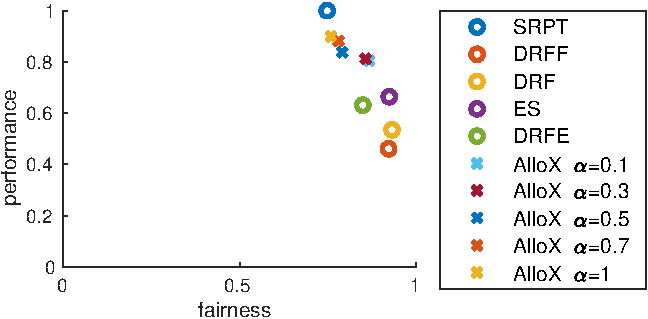
\includegraphics[width=1.0\linewidth]{figs/perf_fair_tradeoffs}
%	\caption{\name improves the performance of average completion time by up to 35\% while maintains fairness level closely to the traditional fair schedulers.}
%	\label{fig:motivation}
%\end{figure}

\desc{Background: rapid growth of machine learning applications, CPU/GPU cluster, ML jobs and other jobs share the same cluster}

In modern computer systems, multiple resources can be used in an interchangeable way to fulfill the same demand. 
In particular, CPUs and (GP)GPUs can be used for the computation in job processing \cite{tensorflow, debunking, coordinating-gpu-cpu, fpga-gpu-cpu}. 
Generally speaking, CPUs are more efficient for complicated computations with a limited number of threads running in parallel. A powerful server nowadays normally has tens of CPU cores~\cite{intel-xeon}. 
In contrast, GPUs are used primarily for highly parallelized yet simple computations. A single GPU can have as many as 5,120 cores~\cite{nvidia-volta}, each of which runs at a lower frequency and supports limited operations. Recently, GPUs are becoming popular for deep learning, massive data mining, and even networking \cite{fpga-gpu-cpu, tensorflow, packetshader}. Noticeably, Google has developed a specialized FPGA-based processor named TPU for its AI system AlphaGo~\cite{tpu}. 
It is common to run jobs on a cluster consisted of interchangeable resources. 

% All these resources, however, are used by multiple users, potentially from different entities, and they share the same physical infrastructure. 
% Examples of such shared environments include Amazon EC2, Microsoft Azure, and Google Compute \cite{ec2, azure, google-compute} as well as private clusters. 
% The system needs to first allocate resources to these users, while satisfying some basic properties, such as sharing incentive (SI), Pareto efficiency (PE), and strategyproofness (SP) \cite{drf}. After receiving the resources, each user can decide how to run her jobs, e.g., first come first served or shortest remaining processing time first~\cite{sjf}.

\desc{Single configuration vs multiple configurations} 

In such clusters, jobs have more than one configurations. 
Traditionally, a job only has the CPU configuration. For instance, if a job needs 1 CPU and 12 GB Memory (MEM), its CPU configuration is (1 CPU, 12GB MEM). 
With the recent progress on machine learning frameworks such like Tensorflow~\cite{tensorflow}, a wide variety of jobs can be executed on both CPUs and GPUs. 
In addition to the CPU configuration, a job has another GPU configuration, such as (1 GPU, 2GB MEM). 
In the state-of-the-art systems, such as Kubernetes~\cite{kubernetes} for containerized applications, users need to specify either the CPU configuration or the GPU one before a job can be processed. 
The job processing time varies a lot under CPU or GPU configurations. 
In Section~\ref{sec:speedup}, we present experimental results to show that different jobs have distinct speedup using GPUs compared to CPUs .

%so it can have 2 configurations: CPU and GPU configurations.
%For example, a job needs <20 CPU cores, 12 GB RAM> or <1 GPU, 2GB RAM>.

%In \name, the system is shared by multiple users, and each user has a sequence of jobs. In some existing work, there are multiple jobs, each consisted of multiple tasks. The similarity is by scheduling and placement of jobs in \name (or tasks in other systems) to optimize performance and fairness for users (or jobs in other systems). 

\desc{Problem: how to effectively schedule different types of jobs}

The \emph{central problem} of this paper is \emph{how to pick the configuration for each job and order the jobs} to optimize performance objectives such as average job completion time while providing fair resource allocations among multiple users. This needs to be done in an online manner with minimal efforts from users.

% \emph{Problem statement.} The goal of \name is to automatically estimate job demand and schedule jobs to maximize performance objectives while providing fair allocations among users. The resource manager for multiple configuration jobs must pick (i) the configuration to use for each job and 
% (ii) the order and placement of jobs to optimize performance and fairness objectives. 

%\zhenhua{I edited the description of the example, but we need an example with a better improvement.}
Consider a simple example in Table \ref{tbl:mov_example}, where two users share a small cluster of two CPUs and two GPUs. 
Each user has 3 jobs queued up at the beginning that can be processed on either CPUs or GPUs with the processing times shown in the last two columns.
% Each job can execute either on CPU or GPU with different completion times.
% The GPU/CPU speed-up rates of jobs are different.
%6 jobs are queued up at the beginning.

% \begin{table}[H]    
% 	\caption{A motivating example.\todo{relabel the job ID and redraw figure 1 in the same style of other figures in the paper.}}
% 	\label{tbl:mov_example}
% 	\begin{tabular}{|c|c|c|c|}
% 		\hline
% 		User & Job ID & Compl. on GPU & Compl. on CPU \\  \hline \hline
% 		User 1 & 1 & 3 & 4 \\  \hline
% 		User 1 & 3 & 1.5 & 4 \\  \hline
%         User 1 & 5 & 1 & 2 \\  \hline
% 		User 2 & 2 & 3 & 3 \\  \hline
%         User 2 & 4 & 2 & 3 \\  \hline		
% 		User 2 & 6 & 1.5 & 2 \\  \hline
% 	\end{tabular}
% \end{table}

% \xiao{I made a new example as below}
\begin{table}[t]
	\caption{A motivating example. PT stands for processing time in minutes. }\vspace{-0.1in}
	\label{tbl:mov_example}
	\begin{tabular}{|c|c|c|c|}
		\hline
		User & Job ID & PT on GPU & PT on CPU \\  \hline \hline
		User 1 & 1 & 10 & 15 \\  \hline
		User 2 & 2 & 8 & 10 \\  \hline
        User 1 & 3 & 10 & 50 \\  \hline
		User 2 & $  $4 & 5 & 75 \\  \hline
        User 1 & 5 & 10 & 15 \\  \hline		
		User 2 & 6 & 10 & 15 \\  \hline
	\end{tabular}\vspace{-0.2in}
\end{table}


\begin{figure}[!htbp]
	\centering
	{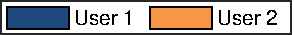
\includegraphics[width=0.45\linewidth]{figs/example_legend} }    \hspace{0.0in} \\
	\subfloat[Equal Share] {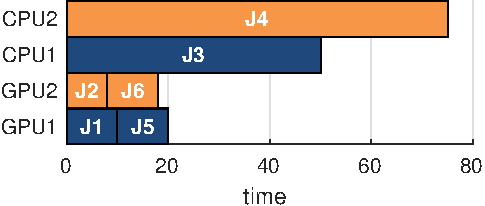
\includegraphics[width=0.7\linewidth]{figs/example_fair} \label{fig:motivation_example_1}}\vspace{-0.1in}    \hspace{-0.1in}
	\subfloat[\name] {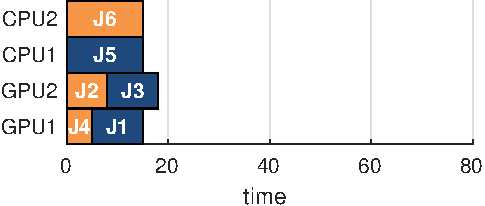
\includegraphics[width=0.7\linewidth]{figs/example_opt} \label{fig:motivation_example_2}}   \vspace{-0.1in} \hspace{-0.1in}		\caption{Improvement from \name scheduling.
}\vspace{-0.2in}
	\label{fig:motivation_example}
\end{figure}

%\xiao{The numbers are $\frac{181}{6}$ vs $\frac{76}{6}$, with around 59\% improvement}

Figure \ref{fig:motivation_example} compares a strawman solution and our solution \name developed in this paper.
The strawman solution in Figure \eqref{fig:motivation_example_1} divides CPUs and GPUs equally between the two users and places the jobs on CPUs and GPUs in a First-Come-First-Served (FCFS) manner. 
When it is the turn for a particular job to run, this job picks its ``favorite'' resource (the one results in shorter processing time) if that resource is available, otherwise it picks the other resource. This equal sharing solution results in an average job completion time of $\frac{181}{6}$ minutes.

%~\todo{How to pick the configuration? What's FCFS given jobs are queued at the beginning?}.  \xiao{To be specific, for each user, we consider the job in order based on the job ID, and we place the job to its favorite device - unless that device is full and there is another device available for that user to schedule the job. For example, for job 3, its favorite device is GPU, but GPU is already full as GPU is being used by job 1, so it has to take CPU}


%The strawman solution fully utilizes the resources but its performance is far from optimal.
Figure \eqref{fig:motivation_example_2} illustrates our solution, which is significantly better.
The average job completion time is reduced to $\frac{76}{6}$ minutes, a $59\%$ improvement. The makespan is also reduced by $76\%$. 


\desc{Motivating example: why interchangeability makes the problem more challenging? (i) average job completion time: SRPT => NP-hard; (ii) resource utilization: work conservation is not good enough; (iii) fairness: DRF is no longer optimal.}

While the improvement is huge, there are significant algorithmic and systems challenges with multiple job configurations. From the performance's perspective, while minimizing the average job completion time is relatively easy when jobs have only one configuration \cite{labetoulle1984preemptive}, the problem is APX-hard when there are multiple configurations by a reduction from a maximum bounded 3-dimensional matching problem \cite{hoogeveen1998non}. %even if we only have two configurations. The proof is from the reduction of \todo{add details}\xiao{look for proving $Rm|pmtn|\sum C_j$ is NP-hard}. When there are arrivals over time, even if the arrival time is known to the scheduler beforehand, the problem becomes APX-hard when there are multiple configurations \todo{add one sentence explanation or point to later section where you have detailed explanations.}. The reduction comes from a maximum bounded 3-dimensional matching problem \cite{hoogeveen1998non}.
%
% ~\todo{Xiao, do you have a detailed explanations?}
% \todo{Show that multiple configurations makes the problem hard }
%
% For example, where there is only one configuration, meaning that only 1 type of resource will be used for computation, the problem is polynomially solvable when all jobs start at the beginning and preemption is allowed, policies like SRPT can tackle these secenarios easily. However, when multiple configurations are allowed, the problem becomes strongly NP-Hard \cite{sitters2001two}, 
% and when there are arrivals - even offline arrivals, meaning that the scheduler knows the arrival times of all jobs, the problem becomes APX-Hard \cite{hoogeveen1998non}.
%
% when there are more than one configurations. For example, for single machine or parallel and identical machine, when all jobs arrives over time, minimizing the average job completion time is relatively easy when each job only has one configuration \cite{afrati1999approximation}. When there are more than one configurations, the problem is equivalent to online scheduling with unrelated machines, where each machine can be viewed as an individual CPU or GPU resource. This problem is APX-Hard \cite{hoogeveen1998non}, even when preemption is allowed. The hardness can be obtained from a Maximum Bounded 3-dimensional matching problem.
%
Regarding fairness, while the Dominant Resource Fairness (DRF) allocation and its variants
~\cite{drf,hug,parkes2015beyond, drfq,choosy,drf_hetor} provide desirable properties, there exists a hard tradeoff among the fundamental properties with multiple job configurations and DRF fails to provide most properties. %That partially explains why strawman solutions in Figure~\ref{fig:motivation_example_1} and later in Section~\ref{sec:perf-strawman} do not work well. 
For system development, existing systems heavily rely on users to provide key information such as which configuration to use in Kubernetes while users may not have the expertise or the system-level information to do so.

We make the following contributions in tackling these challenges by designing \name. 

\begin{itemize}
\item Motivated by experimental results on a real system, we identify a new job scheduling and resource allocation problem and analyze the inefficiencies of existing solutions (\S\ref{sec:background}). Specifically, most existing solutions may lead to \emph{arbitrarily} poor performance when jobs have multiple configurations. %, and the widely used DRF allocation fails to provide most desirable properties . 
\item We design the \name algorithm to optimize performance and provide dynamic fair allocation (\S\ref{sec:alg}). Our key idea is to transform the multi-configuration job scheduling problem into a min-cost bipartite matching problem, which can be solved in polynomial time. It provides the optimal solution in simplified settings and outperforms all baselines significantly in general settings. \name dynamically schedules jobs from the users with the lowest progress for fairness.
%We discuss the new implications of the properties in {\name} and show that it is impossible to achieve SI, SP, and PE simultaneously in \name in \S\ref{sec:fairness}.
\item We implement \name on Kubernetes (\S\ref{sec:system}). Besides the scheduling algorithm, \name profiles jobs in an online manner to automatically decide job configurations and estimates job processing times under different configurations. Both are necessary inputs for the scheduling algorithm. 
\item We conduct experimental and numeric evaluations to show the performance improvements (\S\ref{sec:evaluation}). Results highlight that \name reduces the average job completion time significantly, provides good fairness among users, and prevents starvation.
\end{itemize}


% Our key idea is to transform the multi-configuration job scheduling problem into a network flow problem


% \begin{figure}[t]
% 	\centering
% 	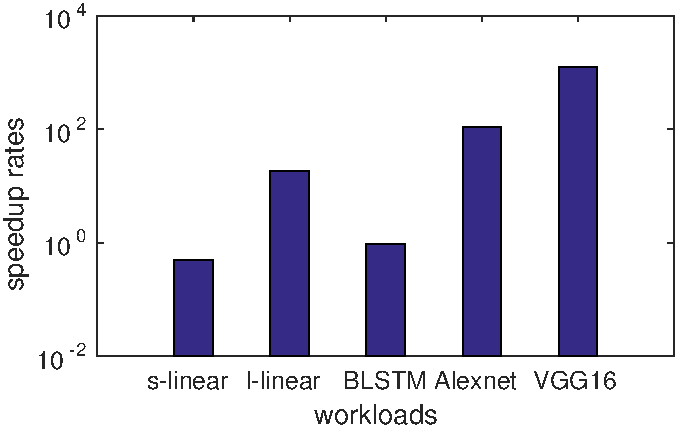
\includegraphics[width=0.7\linewidth]{figs/beta}
% 	\caption{Jobs have different speed-up rates when running on GPUs.}
% 	\label{fig:beta}
% \end{figure}

% % In this paper, we consider the interchangeable resource allocation (\name) problem to decide how to allocate interchangeable resources to multiple users while satisfying the desired properties.  
% % In the new {\name} problem, traditional multi-resource allocation policies such as DRF~\cite{drf} and its variants~\cite{beyond-drf, choosy, hdrf, hug} do not work. In particular, we show that a straightforward application of DRF to \name fails to provide SI, SP, or PE properties. 



% This paper is the first step towards understanding and analyzing this general case. We aim to answer the following questions: (i) Is it possible in {\name} to provide those properties satisfied in the traditional multi-resource allocations? (ii) Can we design efficient algorithms to achieve (or approximate if (i) is impossible) these properties? (iii) How much performance improvements can these algorithms get?




% \desc{Opportunity: CPU low utilization (forward pointing to later figure), identify job types and place jobs on CPU or GPU accordingly}

% Existing systems such as Kubernetes ask users to decide job demand and where to place the job, CPU or GPU~\cite{yarn, kubernetes, mesos}, to simplify the design of schedulers. However, users may not have enough expertise or information to make such choices, leading to significant inefficiencies as shown in Section~\ref{sec:background}. 
% When we allow users to choose the configurations to run their jobs in hybrid CPU/GPU clusters, it may easily result in one of resource become the bottleneck.
% When most people think GPUs are the better resources for them, GPUs can be overloaded while CPUs are abundant and mostly under-utilized like Figure \ref{fig:avg_util}.

% \desc{Our idea: periodic scheduling for fairness, network algorithm for multiple configurations, online profiling for information (explain the importance of having the information)}

% The key motivation for this work is that different users and applications may have dramatically different efficiencies in utilizing GPU for computation.
% Figure~\ref{fig:beta} illustrates results from real experiments.  We start from a simple workload such as linear regression \cite{tensorflow-examples} and consider standard benchmarks such as AlexNet and VGG16 \cite{tensorflow-benchmark}. We consider two linear regression jobs, i.e., s-linear and l-linear, where s-linear has only 200 data points for training and l-linear has 10000 data points. Bidirectional long-short-term memory (BLSTM) is the deep learning architecture that works well with text data ~\cite{deep-learning-cpu-gpu-benchmark}. AlexNet and VGG16 are both well-known convolution neural network (CNN) models. The numbers show how much speedup one GPU (Tesla P100 16GB) can bring compared to only using one physical CPU core (E5-2670 v3 @ 2.30GHz). While GPU is very efficient in accelerating computations (1 GPU can speedup the computation by 1230 times) for applications such as VGG16, AlexNet~\cite{tensorflow-benchmark}, and l-linear~\cite{tensorflow-examples}, it is not very useful for other applications such as s-linear~\cite{tensorflow-examples} and BLSTM~\cite{deep-learning-cpu-gpu-benchmark}.
% We discuss the detailed conversion from GPU to CPU in \S\ref{sec:background}.

% At a high level, we can use a $n\times n$ matrix $\mathbf{E}$ to represent a system of $n$ resources, where the element $e_{ij}$ represents how efficiently resource $i$ can be replaced by resource $j$.
% Then single resource allocation only deals with a $1\times1$ matrix, while the traditional multi-resource allocation extends it to an identity matrix. {\name} works with a general matrix which is not necessarily diagonal. %\todo{add a figure}


%Contributions: (i) identify the problem; (ii) efficient algorithm design; (iii) system implementation and evaluation

	\section{Background \& Motivation}
\label{sec:background}

\subsection{Interchangeable resources}
\label{sec:speedup}

\desc{GPUs are designed for heavy computing applications}

% GPUs become more important than ever because of the rapid increase in compute-intensive applications.
Modern GPUs are not only graphics processors but can also process massive data in parallel using hundreds or thousands of reduced-instruction-set cores.
Consequently, GPUs have been in wide use for deep-learning applications like image classification, video analytics, speech recognition, and natural language processing \cite{image_classfication_deep,image_classification_cnn,cuda_video_coding, nn_nlp, deep_cnn_nlp}.

% \begin{figure}[h]
% 	\centering
% 	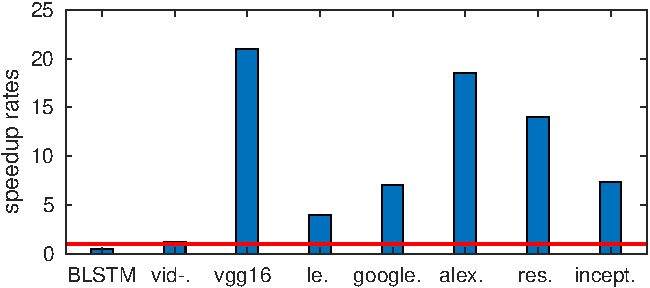
\includegraphics[width=1.0\linewidth]{figs/speedup_rates} \vspace{-0.2in}\caption{Jobs have different speedups from Nvidia K80 GPU versus Intel Xeon E5 2.4 GHz 20-core CPU.}\vspace{-0.1in}
% 	\label{fig:speedup_rates}
% \end{figure}

\desc{GPUs are not always cost effective.}

Different jobs obtain distinct speedups by using GPUs versus CPUs, as shown in Figure~\eqref{fig:speedup_rates}. The speedup rate is how much GPU can reduce the job processing time, i.e., job processing time on a particular CPU divided by that on one GPU. 

While GPUs are generally more efficient for machine learning jobs (with a speedup rate larger than 1), they are more expensive. Figure~\eqref{fig:cost_perf} shows that the normalized costs (the cost ratio between GPUs and CPUs divided by the speedup) vary a lot. When the normalized cost is greater than 1, using GPU is not cost-effective. 

\begin{figure}[h]
	\centering
	%    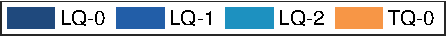
\includegraphics[width=0.6\linewidth]{fig/b1i3_res_usage_legend} 
	\subfloat[Speedups from Nvidia K80 GPU versus Intel Xeon E5 2.4 GHz 20-core CPU.] {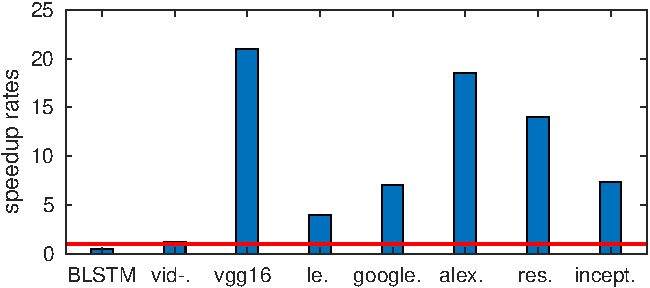
\includegraphics[width=1.0\linewidth]{figs/speedup_rates} \label{fig:speedup_rates}}    \hspace{0.0in}
	\subfloat[Normalized costs using CPUs (c5.large) versus GPU node (p2.xlarge) on EC2] {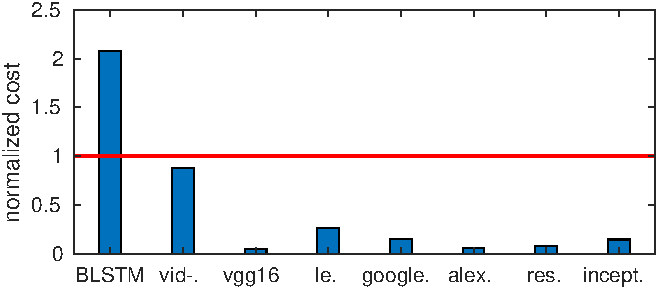
\includegraphics[width=1.0\linewidth]{figs/cost_perf_cloud} \label{fig:cost_perf_cloud}} 
	\caption{GPUs provide distinct speedup and cost-effectiveness.}
	\label{fig:cost_perf}
\end{figure}



%Despite their increasing popularity, GPUs are not always cost effective.
%Figure~\ref{fig:cost_perf} shows normalized costs of CPU and GPU on different benchmarks running on TensorFlow.
% We consider both their off-the-shelf prices and prices on Amazon EC2.
% The normalized cost is the ratio of the GPU price and CPU price, further divided by the speedup rate. The speedup rate is how much GPU can reduce the job processing time, i.e., job processing time on a particular CPU divided by that on one GPU. 
% While GPUs are generally more efficient for machine learning jobs (with a speedup rate larger than 1), they are more expensive. 
% If the normalized cost is more than 1, using GPU is not cost-effective. 

The ineffectiveness of using GPUs in some jobs is due to several reasons.
Although TensorFlow can speedup the performance of CNN models like VGG16, ResNet50, AlexNet, and Inception3 using GPUs \cite{tensorflow-benchmark}, it does not work well with memory networks like Bidirectional LSTM (Bi-LSTM) \cite{deep-learning-cpu-gpu-benchmark}.
RNN models are often updated for each training example for the dependency between two time frames which creates difficulty for parallel computing \cite{huang2013accelerating}.
For the large data input like video-analytics (vid.) \cite{keras-video-classifier}, GPUs are not effective due to the bottleneck in memory and I/O. Therefore, CPUs are preferred for the pre-processing of the video data for the deep learning models.

%\begin{figure}
%	\centering
%	\includegraphics[width=0.7\linewidth]{figs/beta_mov}
%	\caption{Tensorflow jobs have different speedup rates on GPUs (Nvidia K80) vs CPU Xeon E5 2.3Gz 20 cores.}
%	\label{fig:beta_mov}
%\end{figure}




% \desc{CPU applications are still dominant in CPU/GPU clusters}
% We also observe that CPU-only applications are still dominant in most clusters.
% Traditional for-CPU applications have been developed over many years, and it is impractical to convert all these applications for GPUs.
% Furthermore, if the applications are I/O bound, GPUs are not useful.
% For example, database queries are often bound by disk, memory, or network I/O \cite{li2016hippogriffdb}.
% Finally, GPU memory is relatively small; thus it can be a bottleneck for memory-bound applications.
% If the applications do not require much computation, developers will not convert them into GPU applications.
% Although GPU demand is increasing, the load from GPU applications are still small compared to the CPU applications.
%\todo{find the ratio of CPU load vs. GPU load.}

%%% We cannot argue GPUs are not cost effective because speed-up to costs rates are still high as CPU with more CPU cores are also very expensive.
%GPUs may not be cost effective.
%We define the performance-cost ratio as $\frac{\text{speed-up rate}}{(\text{price of GPU}/\text{price of CPU})}$.
%Nvidia shows that Nvidia Tesla K80 can speed-up up to 10x against Intel Xeon E5v3 3.6 Ghz \cite{gpu-k80-speedup}.
%The price of GPU Nvidia Tesla K80 is \$3990 \cite{} while the price of Intel Xeon E5v3 3.6 Ghz is \$363.5 \cite{}.
%
%\begin{figure*}[h]
%    \centering
%    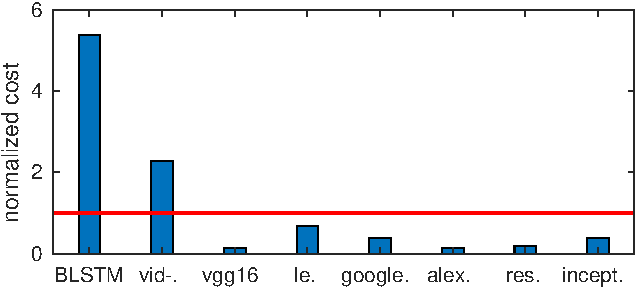
\includegraphics[width=1.0\linewidth]{figs/cost_perf_physical}
%    \caption{Performance-cost ratios show GPUs are not cost-effective because most of ratios are less than 1. Nvidia claims that the speed-up rates of using Nvidia Tesla K80 speeds up 1-10x \cite{gpu-k80-speedup} against Intel Xeon E5v3 3.6 GHz. The price of GPU is \$3990, while the price of CPU is \$363.5.}
%    \label{fig:cost_perf_physical}
%\end{figure*}

\desc{Traditional CPU clusters are low in utilization that gives space for running GPU workloads on CPU.}

In addition to being cost-effective for some jobs, CPUs are often under-utilized.
To this end, we analyzed the Azure Public Dataset \cite{AzurePublicDataset}, which recorded CPU utilization of 5,958 users over 30 days.
We found that more than 90\% users use less than 20\% of their allocated CPU (Figure~\ref{fig:avg_util}).
Because jobs can be executed on CPUs when GPUs are busy, we could utilize the available CPUs before spending a lot in adding more, expensive GPUs.

\begin{figure}[h]
	\centering
	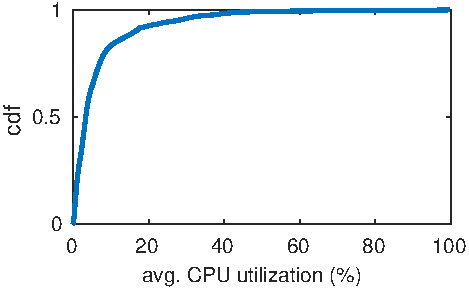
\includegraphics[width=0.8\linewidth]{figs/avg_util}
	\caption{Most of Microsoft Azure users (92.6\% of 5,958 users) have average CPU utilization under 20\%.}
	\label{fig:avg_util}
\end{figure}


\desc{There are interchangeable resources.}

% Thanks to frameworks like TensorFlow \cite{tensorflow}, machine learning applications can run on both CPUs and GPUs.
% Meaning, GPUs can be interchanged with CPUs and vice versa.
% Interchangeable resources like CPUs and GPUs are not rare in large heterogeneous clusters: 
% Heterogeneous CPUs can be interchanged because a more powerful CPU can give better performance than the weaker ones.
% Similarly, one can interchange different network interfaces with different bandwidths, and SSDs with HDDs.

%\subsection{Limitations of current schedulers for CPU/GPU clusters}

\desc{Cannot handle interchangeable resources.}

Unfortunately, existing cluster schedulers do not support interchangeable resources (Table~\ref{tbl:schedulers}) and it is not easy to extend existing schedulers to handle both performance and fairness in the presence of multiple configurations.
Usually, jobs are pre-configured to run on either CPUs or GPUs, therefore systems do not have the flexibility to determine whether to place a job on CPU or GPU. For example, jobs preferring to use GPUs may wait in the GPU queue for a long time, even if CPUs are available and could be a better option in some cases.
Moreover, the configurations are pre-configured by users, who may not know the system-level information to choose the right configurations.


\begin{table}[h]	
	\caption{Resource allocation systems that support GPUs.}
	\label{tbl:schedulers}
	\begin{tabular}{|p{3.5cm}|c|c|}
		\hline
		Systems &  Schedulers & Interchangeability \\ \hline \hline		
		Apache YARN \cite{yarn}    & Fair, DRF & No    \\ \hline
		Kubernetes \cite{kubernetes} & Best effort & No \\ \hline
		Apache Mesos \cite{mesos}   &  DRF          & No  \\ \hline
		Apache Spark \newline (Standalone Mode) \cite{spark}   &  Fair         & No  \\ \hline
	\end{tabular}\vspace{-0.2in}
\end{table}

\desc{Fixed Resource placement is not efficient}

%Since the resource configuration of a job is fixed before its submission, resource interchangeability becomes impossible.


\subsection{Inefficiencies of strawman solutions}
\label{sec:perf-strawman}
%\xiao{new idea: consider the load. When the load is low, actually both MEC and JSQ+ are optimal. But when the load increases, there is a problem. Our approach shirinks to JSQ+ or MEC when the load is low, but when load increases, we have better performance}


\desc{Problem Definition}
To better understand the shortcomings of simplistic heuristics, let us consider a simple setup. 
Assume there are $n$ users sharing a system consisted of interchangeable resources, where each user submits their jobs over time. 
Each job has up to $k$ configurations to run. 
For simplicity of presentation, we restrict our attention to two configurations, i.e., the GPU and the CPU configurations; however, our algorithm and analysis can be readily extended to more configurations, and  different scenarios such as networking interfaces or storage devices. 
A job scheduler for interchangeable resources needs to decide 
(i) the configuration to use for each job and 
(ii) the order of jobs to optimize performance and fairness objectives. 

By default, we do not allow preemption because it is not well supported in many systems such as Kubernetes. 
Even if it is supported, the overhead of migration is often very high. 


%% tan: deletes this example because it does not help.
\del{
Consider a simple example where there are 1 CPU consisted of 32 cores and 1 GPU in the system. 
Each job has two configurations: either the whole CPU or the whole GPU (with a small amount of CPU, e.g., less than a core, to ensure normal execution). 
There are two users. 
User 1 has 5 jobs, each takes 10 minutes to finish on CPU, and 5 minutes on GPU. User 2 has 5 jobs requires 40 and 10 minutes on CPU and GPU, respectively. 
If we want to minimize the average job completion time (JCT), the optimal solution is to put all jobs of user 1 on CPU and all jobs of user 2 on GPU, resulting in an average JCT of 30 minutes. 
}


%processing time on CPU, or 5 mins on GPU, while Job 2 requires either 40 mins processing time on CPU or 10 mins on GPU. If we try to minimize the average completion time, then clearly we should use GPU for job 2 and CPU for job 1.





%Each version will use corresponding GPU or CPU as the computational resource, and each job can only pick one configuration. Assume every job has the same configuration settings, but the processing time on different resources are different, and we assume the processing time is known. The goal is to decide the configuration for each job and then schedule the jobs to reach a better performance and fairness output.

While (ii) has been studied extensively in existing work~\cite{drf,drfq,carbyne,tetris,hug}, (i) is the new challenge. 
In this section, we revisit existing algorithms for this new problem to illustrate their inefficiencies and demonstrate why we need new algorithms. 
In addition, we show that strawman solutions may lead to poor performance, highlighting that designing a new algorithm is challenging.






%In the following subsection, we will consider performance (in terms of job completion time) and fairness seperately. We will see that a strawman solution fails to solve this problem -  and in most of the time, far from optimal solution.

%\subsubsection{Performance}

We focus on performance in this section, in particular, minimizing the average job completion time (JCT). Fairness is discussed in Section~\ref{sec:fairness}.  

\desc{Each job use its most effective resource}

%For the problem described above, if our goal is to minimize average completion time, the problem is in P if we assume all jobs arrives at time 0. if they arrive over time, then the problem becomes strongly NP-Hard, even if we allow preemption. Before we discuss our polynomial algorithm in section xxx, we start with heuristics and show why they did not work.


The first approach we consider is Most Effective Configurations (MEC): the scheduler asks users to pick one configuration for each job and the scheduler is only responsible for the job ordering and placement. 
Under this approach, the load on CPU and GPU can be largely unbalanced. For instance, if all jobs favor GPUs, no users would pick the CPU configuration, resulting in arbitrarily low utilization of CPU, and vice versa. 
Actually, if there are $k$ interchangeable resources, this approach may result in $k-1$ of them unused. 

The under-utilization of resources has profound impacts on job completion time, especially when the system load is high. For instance, assume all the GPUs together can finish 10 jobs/minutes on average and all the CPUs can finish 10 jobs/minutes possibly with longer processing time for each job. Then if the arrival rate is 15 jobs/minutes, the waiting time when we only use GPUs would keep increasing. Under the ``heavy traffic'' situations, low utilization results in arbitrarily large job completion time. 
%\del{, and these situations are exactly when we greatly need thoughtful scheduling algorithms}.
Therefore, \emph{picking the most effective configuration for each job may result in low utilization and high waiting time}.

%This approach is not optimal, as the load of CPU and GPU can be largely unbalanced, especially for machine learning jobs. For example, if for all jobs, the processing time on GPU is always shorter than CPU, then of course people would choose using GPUs in a shared cluster. While GPU is fully utilized, CPUs are barely used. So the performance can be as bad as the computational power between total GPUs and total CPU cores. For example, if they have the same computational power, then the degeneration can be as much as 50\%.

\desc{users see the load}

The inefficiency of MEC is because the configuration selection does not take into consideration the current system load. Therefore, the second approach is a modified Join the Shortest Queue (JSQ+). 
Assume users know the current waiting time on each resource in real time. On the arrival of a job, the scheduler picks the resource that has the shortest completion time, i.e, the sum of waiting time and the processing time of the job on the corresponding resource. 
In this way, loads on different resources can be more balanced because as the load on some resources increases, their longer waiting time would encourage new jobs to be placed on other resources. 
Note that it is different than the vanilla joining the shortest queue. 
For instance, if a job has the processing times of 10 minutes and 40 minutes on GPU and CPU, respectively, and the waiting times on GPU and CPU are 40 and 20 minutes, respectively.
Although CPU has a shorter waiting time, this job pick GPU because it is much more efficient on GPU, resulting in a completion time of 50 minutes.
If the job was placed on CPU, the completion time would increase to 60 minutes.

%reports back the current node on different resource - so the user can choose whichever node that has the shortest expected finishing time if the job will be running on that node. 

\emph{The key drawback of JSQ+ is that it is short-sighted}: each job attempts to minimize its own completion time without considering the impacts on later jobs. 
Here is an example with 2 CPUs and 2 GPUs. Assume there are 4 jobs, all arrive at the beginning but in the order of Job 1, 2, 3, 4. The processing time can be show in a matrix: 
$$
P = \begin{bmatrix}
40 & 50 \\
40 & 50 \\
40 & 80\\
40 & 80\\
\end{bmatrix}
$$
In this matrix, the $i$-th row consists of job $i$'s processing times on GPUs and CPUs, respectively. For instance, the first row means Job 1 needs 40 minutes on GPU or 50 minutes on CPU.

Under JSQ+, Job 1 first picks a GPU, and then Job 2 picks the other GPU.
After that, Job 3 and Job 4 have no choices but to pick CPUs, as shown in Figure~\eqref{fig:JSQ_ex} with an AJCT of 60 minutes.
%\xiao{This may not be true, as Job 3 and 4 can choose to join the GPU queue and wait instead of using CPU directly}
Clearly, the optimal solution is to put Job 3 and 4 on GPUs and Jobs 1 and 2 on CPUs, which can reduce the AJCT from 60 minutes to 45 minutes as Figure \eqref{fig:JSQ_ex_opt}.

\begin{figure}[h]
	\centering
%	{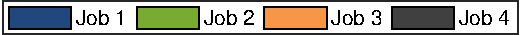
\includegraphics[width=0.7\linewidth]{figs/JSQ_ex_legend} \label{fig:JSQ_ex_legend}}    \hspace{0.0in}
	\subfloat[JSQ+] {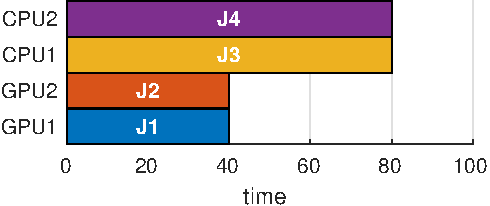
\includegraphics[width=0.7\linewidth]{figs/JSQ_ex} \label{fig:JSQ_ex}}    \hspace{0.0in}
	\subfloat[Optimal] {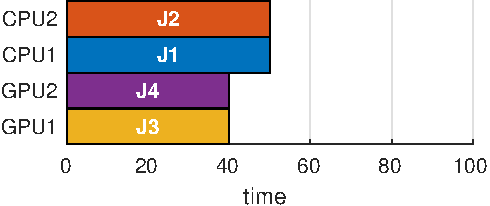
\includegraphics[width=0.7\linewidth]{figs/JSQ_ex_opt} \label{fig:JSQ_ex_opt}}    \hspace{0.0in}	
	\caption{Under JSQ+, Job 1 and 2 are scheduled on GPU, while Job 3 and 4 are scheduled on CPU. In contrast, \name runs Job 3 and Job 4 on GPUs because they have higher speedup on GPUs. } %\tanle{We don't need 4 jobs in the motivation examples. Should I make it to two jobs or vary the lengths a bit?}}
	\label{fig:JSQ}
\end{figure}

%Clearly, this is not an optimal solution, as there is more gain by scheduling Job 3 and 4 to GPUs.


\desc{System pick configuration}

The sub-optimality of these two strawman solutions implies that we cannot just let each user pick her own job configurations, even if users are equipped with the current system load information. 
Therefore, the scheduler needs to coordinate the decisions, where Shortest Job First (SJF) is widely used.
%So now we consider a centralized approach by comparing all configurations between jobs. 

When there are multiple configurations for each job, we can extend SJF to SJF+ to handle jobs with multiple configurations: for each type of resource, maintain a queue of all available jobs. The jobs are sorted based on the processing time on this resource, e.g., GPU, in an increasing order. Whenever a resource becomes available, schedule the first job in the corresponding queue to this resource and remove the job from all queues. When multiple resources are available at the same time, first schedule a job to the one with shorter processing time. 

This algorithm is optimal when there is only 1 configuration~\cite{cobham1954priority}. 
%\todo{Xiao, can you add the citation?}
When there are more than 2 configurations, however, the performance can be \emph{arbitrarily bad}. Consider the following example:

$$
P = \begin{bmatrix}
10 & 20\\
10 & 20 \\
20 & 90\\
20 & 90\\
\end{bmatrix}
$$


\begin{figure}[h]
	\centering
%	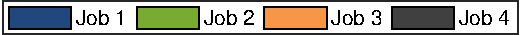
\includegraphics[width=0.7\linewidth]{figs/SJFplus_ex_legend} \hspace{0.0in}
	\subfloat[SJF+] {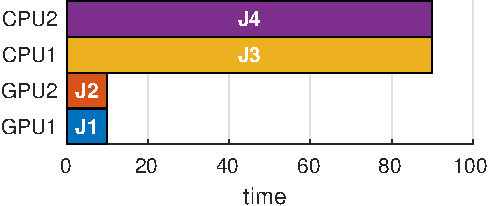
\includegraphics[width=0.7\linewidth]{figs/SJFplus_ex} \label{fig:SJFplus_ex}}    \hspace{0.0in}
	\subfloat[Optimal] {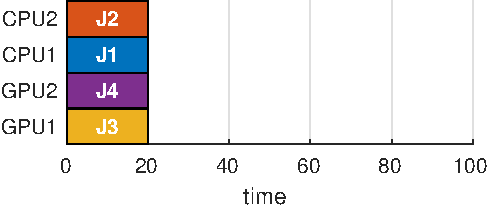
\includegraphics[width=0.7\linewidth]{figs/SJFplus_ex_opt} \label{fig:SJFplus_ex_opt}}    \hspace{0.0in}
%	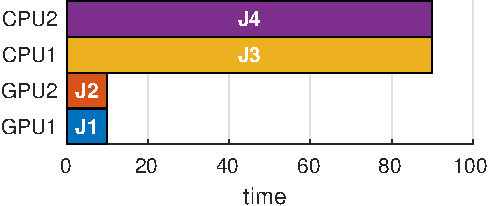
\includegraphics[width=0.8\linewidth]{figs/SJFplus_ex}
	\caption{Under SJF+, Job 1 and 2 are scheduled on GPU, while Job 3 and 4 are placed on CPU. In contrast, \name places Job 3 and Job 4 on GPUs because the time reductions on GPUs of these two jobs are larger.}
	\label{fig:SJF}
\end{figure}


Under SJF+, there are two queues for GPU and CPU, respectively. The order in both queues is Job 1, Job 2, Job 3, Job 4. Therefore, Job 1 and 2 are placed on GPUs first. Then Job 3 and 4 are scheduled on CPUs. This is shown in Figure~\ref{fig:SJF}, resulting in an AJCT of 50 minutes. 
%Job 3 and 4 are large jobs and they have more gains by putting them into GPUs, however, because of the non-idle property of SJF scheduling, Job 3 and 4 are forced to be scheduled on an inefficient resource.
In contrast, the optimal solution places Jobs 3 and 4 on GPUs and Jobs 1 and 2 on CPUs, reducing the AJCT to 20 minutes. 
The root cause is while Jobs 3 and 4 are longer (disadvantage in SJF+), the processing time reduction of using GPU is much larger (overlooked by SJF+).


To summarize, when jobs have multiple configurations, even if jobs arrive at the same time, the problem is more challenging than that with single configuration because we need to consider the processing time reduction among different configurations, which may contradict with other factors, e.g., the length of the job. Therefore, algorithms that perform well for single configuration job scheduling may result in arbitrarily bad performance in the new problem.  

%with 2 configurations for each job, all existing heuristics failed to provide a good guarantee, even for the simplest case. The root is that, it seems to have more gains, we should schedule large jobs on efficient resource, but from traditional scheduling perspective, to minimize average completion time, we should start with smaller jobs. 


In \S\ref{sec:alg}, we will provide a network algorithm, and show its optimality for average job completion time.





% \subsection{Illustrations of \name}

% \desc{Strawman solutions do not work.}

% To handle interchangeability, a strawman solution would equally shares the resources among users and then places the jobs into resource in the best-effort manner.
% To illustrate the inefficiency of the strawman solution and the potential of \name, we create an simple example in Table \ref{tbl:mov_example}.
% There are 2 users, i.e., User 1 and User 2.
% Each user has 3 jobs.
% Each job can execute either on CPU or GPU with different completion times.
% The GPU/CPU speed-up rates of jobs are different.
% 6 jobs are queued up at the beginning.

% \begin{table}[H]    
% 	\caption{Motivation example.}
% 	\label{tbl:mov_example}
% 	\begin{tabular}{|c|c|c|c|}
% 		\hline
% 		User & Job ID & Compl. on GPU & Compl. on CPU \\  \hline \hline
% 		User 1 & 1 & 3 & 4 \\  \hline
% 		User 2 & 2 & 3 & 3 \\  \hline
% 		User 1 & 3 & 1.5 & 4 \\  \hline
% 		User 2 & 4 & 2 & 3 \\  \hline
% 		User 1 & 5 & 1 & 2 \\  \hline
% 		User 2 & 6 & 1.5 & 2 \\  \hline
% 	\end{tabular}
% \end{table}

% Figure \ref{fig:motivation_example} compares the strawman solution and \name.
% The strawman solution in Figure \ref{fig:motivation_example_1} equally shares CPU and GPU for two users and places the jobs in CPUs and GPUs.
% The average completion time of 6 jobs in Figure \ref{fig:motivation_example_1} is $\frac{20}{6}$.
% The strawman solution fully utilizes the resources but its performance is far from optimal.
% Figure \ref{fig:motivation_example_2} illustrates our solution that is clearly better than the strawman one.
% The average completion in Figure \ref{fig:motivation_example_2} is $\frac{13}{6}$ that achieves $35\%$ performance improvement.

% \begin{figure}[H]
% 	\centering
% 	% 3+4+3+5+2+3
% 	\subfloat[Fair share \& Best effort] {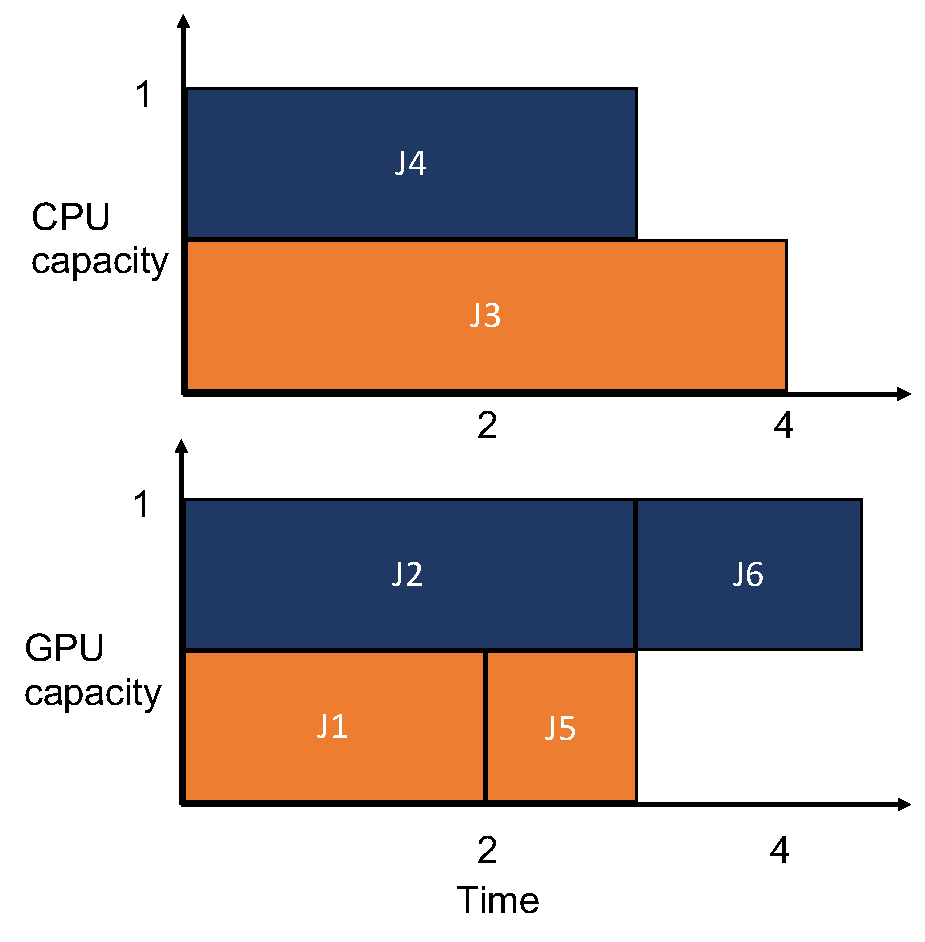
\includegraphics[width=0.45\linewidth]{figs/motivation_example_1} \label{fig:motivation_example_1}} 
% 	% 3+2+1.5+3+1+2.5
% 	\subfloat[\name allocation \& scheduling ]{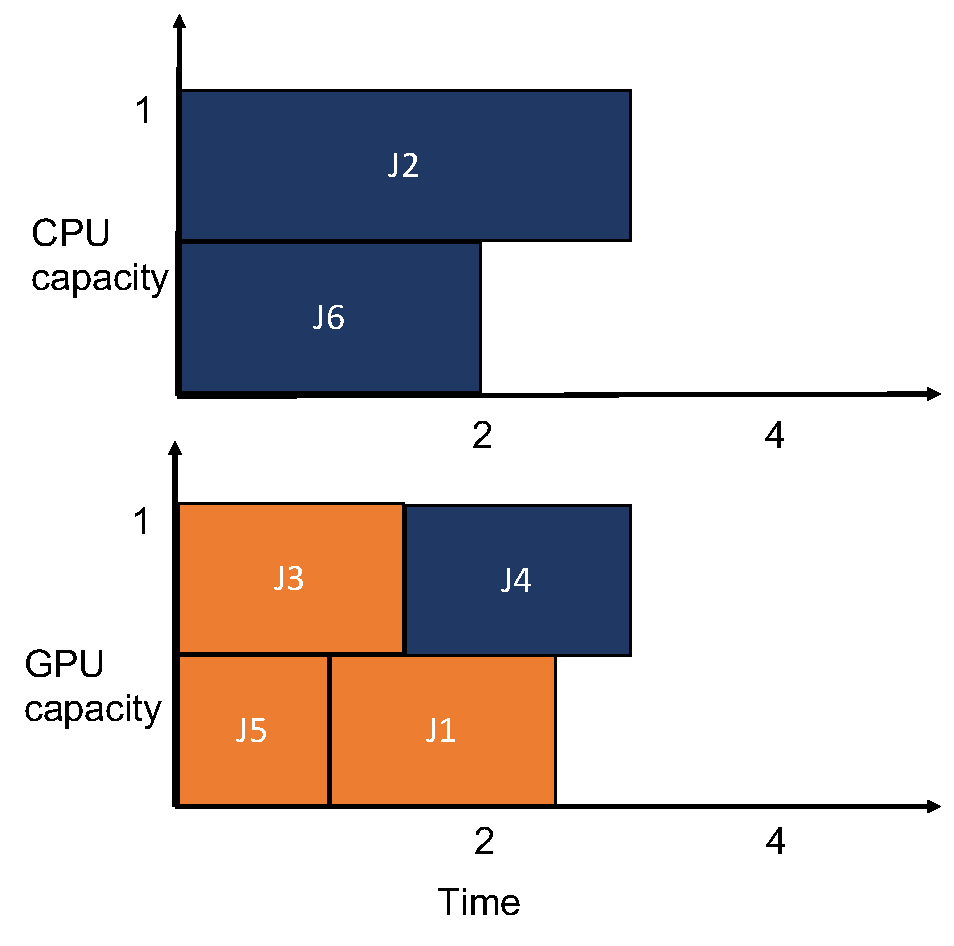
\includegraphics[width=0.45\linewidth]{figs/motivation_example_2} \label{fig:motivation_example_2}}
% 	\caption{Opportunities for job scheduling in CPU/GPU clusters.
% 	Figure \ref{fig:motivation_example_1} depicts the allocation of the strawman solution using fair-share and best-effort scheduling in the FIFO maner.
% 	Although the strawman solution fully utilizes resources, it does not give the optimal solution.
% 	Meanwhile, \name exploits the interchangeability between CPUs and GPUs to improve 35\% performance.}
% 	\label{fig:motivation_example}
% \end{figure}

% \xiao{Motivation starts here} \\
% As our goal is manifold: fairness, efficiency and performance, we show that current existing schedulers and algorithms fail to provide satisfiable result in at least 1 or more aspect.



%This approach works well in the offline case where we can perfect measure the $\beta$. If the $\beta$ is properly choose, we can prove that this algorithm is Pareto-efficient, Envy-free and sharing-incentive. 

%However, under online case, we can not get perfect $\beta$, and the estimation will be changing overtime, so the dominant share of all users are fluctuating, thus those properties can hardly hold in online case.

% \subsubsection{Efficiency}

% In traditional multi-resource allocation problem, the efficiency, or the system utilization is often optimized based on some greedy 'packing' heuristics. As long as the resource is not wasted at every time slot, we should observe a better makespan, so that the efficiency will be improved.  However, under \name, this is no longer true due to job placement onto an improper computation resource. Consider the following example:

% Assume the cluster size is (24 CPU cores, 2 GPUs and 48 GB memory) there is only 1 user in the system and the user has 2 different categories of jobs. 9 jobs are from Type A, which require 8 CPU cores and 8 GB memory, with 10 units processing time and 1 GPU and 2 GB memory with 3 units processing time. 2 jobs are from Type B, which require 16 CPU cores and 16 GB memory, with 8 units processing time on CPU and 1 GPU and 2 GB memory with 30 units processing time.

% The comparison of a packing scheduler and a non-packing scheduler is shown at figure \ref{fig:efficiency}.
% \begin{figure}
% 	\centering
% 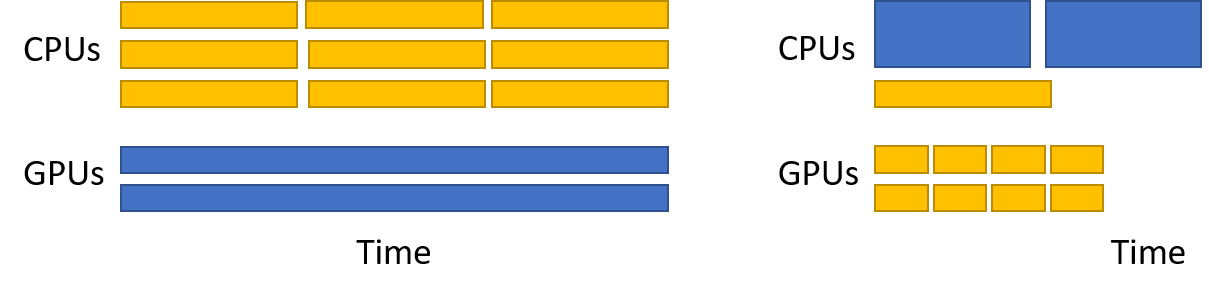
\includegraphics[width=0.8\linewidth]{figs/efficiency}
% 	\caption{Perfect packing does not leads to good utilization. The makespan for left figure is 30, and it is 16 for right figure with imperfect packing.}
% 	\label{fig:efficiency}
% \end{figure}


% \subsubsection{Performance}
% The performance evaluated for a user is based on the average completion time of all jobs from that user. Usually for this objective function,  the widely applied heuristic policy is shortest  job first - simply sort all jobs and schedule the job with shortest processing time. We show that simple vanilla greedy SPT algorithm would also face challenges under our interchangeable settings.

% Similar to previous setting, assume we have a cluster of size (24 CPU cores, 2 GPUs and 48 GB memory) and there is only 1 user in the system, so we don't have to consider fairness. There are 2 types of jobs, all of them have identical job demand but have different processing time. For type A jobs, they require 8 time units on both CPU and GPU. For type B jobs, they require 10 units on GPU and 20 units on CPU. The schedule for SPT and optimal is shown at Figure \ref{fig:performance}.

% \begin{figure}
% 	\centering
% 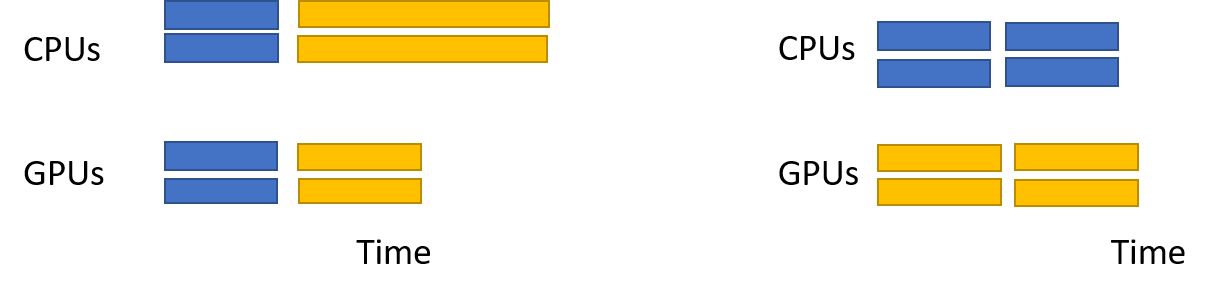
\includegraphics[width=0.8\linewidth]{figs/performance}
% 	\caption{SPT is not necessarily optimal. The ACT for SPT is 15.5 while the act for optimal is  13.5.}
% 	\label{fig:performance}
% \end{figure}

% \subsection{Modeling}

% We model our \name allocation and scheduling problem starting from the workload. In a typical hybrid cluster, assume $C_1,C_2,C_3$ represents the capacity of CPU cores, GPUs and memory from the cluster. there are $n$ active users, and each of them keep submitting machine learning jobs. For each job $j$, when it arrives at time $r_j$, it contains 2 configurations representing the resources demand  
% $$
% 	Q_i=
% 	\begin{bmatrix}
% 	c_i & m_i^1 & p_i^1 \\
% 	g_i & m_i^2 & p_i^2 
% 	\end{bmatrix} $$
% where the first row shows the demand and estimated processing time if the job  will be placed in CPU and the second row show the corresponding GPU configurations.

% Consider the  non-preemptive offline scheduling problem first, the constraints can be formulated as the following:

% \begin{equation}
% \begin{array}{ll@{}ll}
% ~ & \displaystyle\sum\limits_{i,s} x_{i,j,s} =1  & \forall j \\
% ~ &  \displaystyle\sum\limits_{j,s\in (t-p_j^i,t]} x_{i,j,s}c_j \leq   C_1  & ~~\forall i,t \\
% ~ &  \displaystyle\sum\limits_{j,s\in (t-p_j^i,t]} x_{i,j,s}g_j \leq   C_2  & ~~\forall i,t \\
% ~ &  \displaystyle\sum\limits_{j,s\in (t-p_j^i,t]} x_{i,j,s}m_j^i \leq   C_3  & ~~\forall i,t \\
% ~& x_{i,j,s} = 0   & ~~\forall i,j,s > T-p_j^i ~or~s<r_j\\
% & x_{i,j,s} = \{0,1\} & \forall i,j,s\\
% \end{array}
% \end{equation}

% with extra trivial nonnegative constraints. In the above integer programming, $T$ is a trivial upper bound on the makespan of any reasonable schedule. $x_{i,j,s}$ indicates whether job $j$ is processed with computation resource $i$ at starting time $s$. 

% The objective function, depending on ACT or makespan, can be formulated as $\sum\limits_{i,s}x_{i,j,s}(s+p_{j}^i)$ or $\max x_{i,j,s}(s+p_{j}^i)$. However, regardless of what objective we choose, the optimization will be a NP-Hard problem. The hardness come from 2 parts: the multi-dimensional queueing problem, and the rigid job scheduling problem. Hence, for current paper, Our goal is to seek heuristic that works well in the real system.





\subsection{Other challenges}



\desc{Simultaneously improve performance, efficiency, and fairness.}

The tradeoff between performance and fairness is well-known \cite{fairness_efficency_tradeoffs,hug}.
For our problem, if we only optimize for performance using ideas such as shortest job first, users with larger jobs may starve so it is not fair at all.
On the other hand, if we aim at instantaneous fairness such as DRF, there is not much room to improve the performance.
Therefore, the key challenge is how to achieve better job completion time with fairness. 

\desc{Need to estimate the performance of job on CPU or GPU}

On the system side, we need to estimate the job completion times in an online manner with reasonable overhead.
This provides inputs for the scheduler in \name and can free users from setting up the configurations. 


% To achieve the improvement in Figure \ref{fig:motivation_example_2}, we  need to have the estimate of completion times of jobs.
% However, performance prediction is challenging \cite{ernest, cherrypick}.
% First, low accuracy may result in largely negative impact on \name.
% Second, prediction may require large overheads which can make the improvement may not be useful.
% In spite of these challenges, we still want to provide this performance prediction with low overheads and high accuracy.

% It is difficult to optimize performance, efficiency, and fairness simultaneouly.
% If we enforce fair resource allocation among users like Figure \ref{fig:motivation_example_1}, it hurts the performance and efficiency.

% To improve performance, the straight-forward solution is to put the jobs with low speed-up rates on CPUs and jobs with high speed-up rates on GPUs.
% However, it is not true that it also maximizes the efficiency and fairness.
% To demonstrate this, we re-use the motivation example in Table \ref{tbl:mov_example}.
% For instance, we place jobs with large speed-up rates $(\geq 1)$ in GPUs, while putting the small speed-up rates $(<1)$ on CPUs.
% In this case, we actually place all 6 jobs on GPUs but do not use any CPUs that results in low efficiency.

% If we try to optimize the performance and efficiency, it is not trivial to maintain fairness among users.
% When resources are interchangeable, it is actually hard to define fairness.
% Traditional schedulers \cite{yarn, mesos} maintain fairness based on the received resources among users.
% However, this definition of fairness cannot be used when resources are not equally important.
% Naive fair allocation may result in inefficiency like Figure \ref{fig:motivation_example_1}.
	\begin{algorithm}
	\small
\caption{\name Scheduler}
\label{algorithm1}
\begin{algorithmic}[1]
\Procedure{periodicSchedule()}{}
\If{there are new {\burstq}s $\mathbb{Q}$}
	\State $\{\mathbb{H},\mathbb{S},\mathbb{E}\}$ =\textsc{LQAdmit}($\mathbb{Q}$)\EndIf
\If{there are new {\batchq}s $\mathbb{Q}$}
	\State $\{\mathbb{E}\}$ =\textsc{TQAdmit}($\mathbb{Q}$)\EndIf
\State \textsc{allocate}($\mathbb{H},\mathbb{S}, \mathbb{E}$)
\EndProcedure
\\
\Function{LQAdmit({\burstq}s $\mathbb{Q}$)}{}
\ForAll{\burstq  $Q \in \mathbb{Q}$}	
\If{safety condition \eqref{eqn:ad-safety} satisfied}
	\If{fairness condition \eqref{eqn:ad-fair} satisfied}
		\If{resource condition \eqref{eqn:ad-enough} satisfied}
			\State Admit $Q$ to hard guarantee $\mathbb{H}$
		\Else
			\State Admit $Q$ to soft guarantee $\mathbb{S}$
		\EndIf
	\Else
		\State Admit $Q$ to elastic $\mathbb{E}$ with long-term fair share

	\EndIf
\Else 
	\State Reject $Q$
\EndIf
\EndFor
\State \textbf{return} $\{\mathbb{H},\mathbb{S},\mathbb{E}\}$	
\EndFunction
\\
\Function{TQAdmit(queue $\mathbb{Q}$)}{}
\ForAll{\batchq  $Q \in \mathbb{Q}$}	
	\If {safety condition \eqref{eqn:ad-safety} satisfied}
		\State Admit $Q$ to elastic $\mathbb{E}$ with long-term fair share
	\Else 
		\State Reject $Q$
	\EndIf
\EndFor
\State \textbf{return} $\{\mathbb{E}\}$
\EndFunction
\\
\Function{allocate($\mathbb{H}$, $\mathbb{S}$, $\mathbb{E}$)}{}
\ForAll{\burstq $Q \in \mathbb{H}$}
\State $\myvec{a_i}(t)=\frac{\myvec{d_i}(n)}{t_i(n)}$ for $t\in[T_i(n),T_i(n+1)]$ %until $Q$'s consumption reaches $\myvec{d_i}(n)t_i(n)$. 
\EndFor
\ForAll{\burstq $Q \in \mathbb{S}$}
\State allocate $\myvec{C}-\sum_{j\in \mathbb{H}}\myvec{a_j}(t)$ based on SRPT until each {\burstq}-$i$'s allocation reaches $\myvec{d_i}(n)$ or the deadline arrives.
\EndFor
\State Obtain the remaining resources $\myvec{L}$
\State DRF($\mathbb{E}$, $\myvec{L}$)
\EndFunction
%\State Reset $\mathbb{E} = \mathbb{E} \cup \mathbb{U}$, $\mathbb{U} = \emptyset$
%\State Sort $\mathbb{E}$ based on queue start time.
%\ForAll{\burstq  $E \in \mathbb{E}$}	
%	\If {short-term conditions \eqref{eqn:shortterm_adm_cond} satisfied}
%		\State Update $\mathbb{U} = \mathbb{U} \cup U$, $\mathbb{E} = \mathbb{E} \setminus E$
%	\EndIf
%\EndFor
%\State \textbf{return} $\{\mathbb{U} ,\mathbb{E}  \}$	
%\EndFunction
\end{algorithmic}
\end{algorithm}

	\subsection{Fairness}
\label{sec:fairness}
%\tanle{organized and shortened this section}

\subsubsection{Existing fair allocations do not work}

When multiple users share the same cluster, fairness is often important in order to provide performance isolation and to avoid starvation. 
In traditional multi-resource allocation problem, where each job has only one configuration, there are four main properties \cite{drf}:

\begin{itemize}
  \item Pareto Efficiency (PE): No user can increase her performance
without hurting the performance of at least another user.

  \item Sharing Incentive (SI): Each user is no worse by sharing
than using $\frac{1}{n}$ of the system resources exclusively.

  \item Envy-Freeness (EF): No user prefers the allocation of another user for better throughput.

  \item Strategy-proofness (SP): No user is able to benefit by lying.

\end{itemize}

% \begin{figure}
% 	\centering
% 	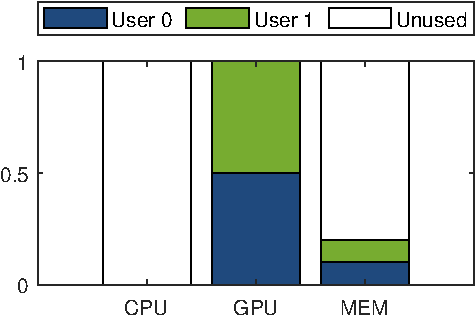
\includegraphics[width=0.7\linewidth]{figs/fairness_ex}
% 	\caption{All CPU cores will remain idle if we allow users to choose their favorite configurations and allocate resource based on DRF. \tanle{this figure is trivial and not referred in the paper --> to be removed.}}
% 	\label{fig:motiv1}
% \end{figure}


DRF \cite{drf} satisfies all four properties when each job has only one configuration. Intuitively, one might expect to extend DRF to the allocation of interchangeable resources. One straightforward extension is to pick the resource configuration with the shortest processing time for each job and then use DRF to allocate the resources by ignoring the interchangeability among resources, e.g., taking CPUs and GPUs as different resource types.
%user estimate their job performance on different resources (CPUs and GPUs), and they demand the resources (one resource from computation and memory) that work the best for that particular job. 
Unfortunately, this does not work. Formally, we have the following lemma regarding this DRF extension.

\begin{restatable}[]{lem}{drf}
	\label{lem:drf_fail}
	If each job picks the configuration with shorter processing time, there exist cases where DRF fails to provide PE, SI or SP under multiple configurations.
\end{restatable}

%\emph{DRF fails to provide SI.}
%However, this approach breaks easily under the simplest setting.
%Assume there are 2 users with identical jobs that prefer GPUs slightly. Both users request GPUs and are allocated half of GPUs, while CPUs are not used. Clearly the sharing incentive is violated as the allocation is worse than equal sharing of all resources between these two users.\mosharaf{Didn't get it.}

Surprisingly, there is a hard tradeoff among these basic properties \cite{sun2018fair}. In particular, we can show for any allocation, if
it provides sharing incentive and Pareto efficiency, it cannot
be strategyproof. Conversely, if it is strategyproof, sharing
incentive and Pareto efficiency cannot be provided simultaneously.
There is one exception: if all jobs have the same speedup by using GPUs, then the problem degenerates to a traditional multi-resource allocation, where DRF can be applied. However, it is not true in practice as shown in Figure~\ref{fig:speedup_rates}. Formally, we have the following impossibility result.

\begin{restatable}[]{lem}{imposs}
\label{lem:imposs}
No multi-configuration allocation can satisfy (i) PE and SI, and (ii) SP simultaneously unless the relative efficiency of CPU and GPU is the same for all jobs. \end{restatable}

%Notice that when relative efficiency of CPU and GPU is the same for all $n$ users, then GPU is equivalent to a faster or slower CPU for all users,  then existing approach can be easily adapted to this case. However, this is not true in reality as shown in Figure \ref{fig:beta}. 

% Interestingly, in current systems, users normally do not know their job characteristics or the system conditions exactly. Therefore, it is hard for users to ``game'' the system. %So strategyproofness seems not necessary.\mosharaf{This doesn't make sense.}
% In addition, we develop an online profiling tool in \name. Therefore, the system no longer requires users to submit their job characteristics.
% %Details can be found in Section ???.
% \mosharaf{ I don't see the point of this discussion.}

% Given the job characteristics estimated by our online profiling tool, another extension of DRF is that: the scheduler sort the jobs based on the relative efficiency on GPUs versus CPUs. 
% Pick a threshold value $b$. If a job's relative efficiency exceeds $b$, pick the GPU configuration. Otherwise, pick the CPU configuration. Then perform DRF by taking CPUs and GPUs as different resource types. 

%The placement will be determined by some fixed threshold value $\beta$, if the efficiency of job $j$ is smaller than $\beta$, it will be placed in CPU, if $j$ is larger than $\beta$, it will be placed in GPU, then the allocation is determined by DRF.


% On the positive side, we have the following result. 

% \begin{restatable}[]{lem}{thresholdDRF} 
% 	\label{lem:thresholdDRF}
% 	If computation is the only bottleneck resource, there exists a threshold-DRF policy that is PE,SI and EF assuming resources are divisible and jobs from the same user are identical.
% \end{restatable}

% However, it is not easy to decide this threshold $b$.
% Especially, when demand changes overtime the threshold is not a constant.
% Moreover, if other resources such as memory can become the bottleneck, any threshold-DRF approach fails to provide desirable properties. More detailed proof is in Appendix \ref{sec:lem:thresholdDRF}
%\mosharaf{I think all these should be relegated to appendix and we should focus on our algorithm.} \tanle{done.}

% Jobs of user $i$ have efficiency 50 while jobs from user $j$ have efficiency 80. The threshold is some value between 50 and 80 so that user $i$'s jobs are placed on CPUs while user $j$'s jobs are placed on GPUs. 
% For jobs of user $i$, assume its CPU configuration is 8 CPU cores and 8 GB memory (we will discuss how to decide the configurations in section ???) and its GPU configuration is 1 GPU and 2 GB memory. Jobs of user $j$ also have GPU configuration with 1 GPU and 2 GB memory. From figure \ref{fig:DRF-threshold}, the allocation is neither SI nor EF. \todo{Why?} \xiao{it is explained in the figure caption, I will update these figures soon using Tan's standard}
% \begin{figure}
% 	\centering
% 	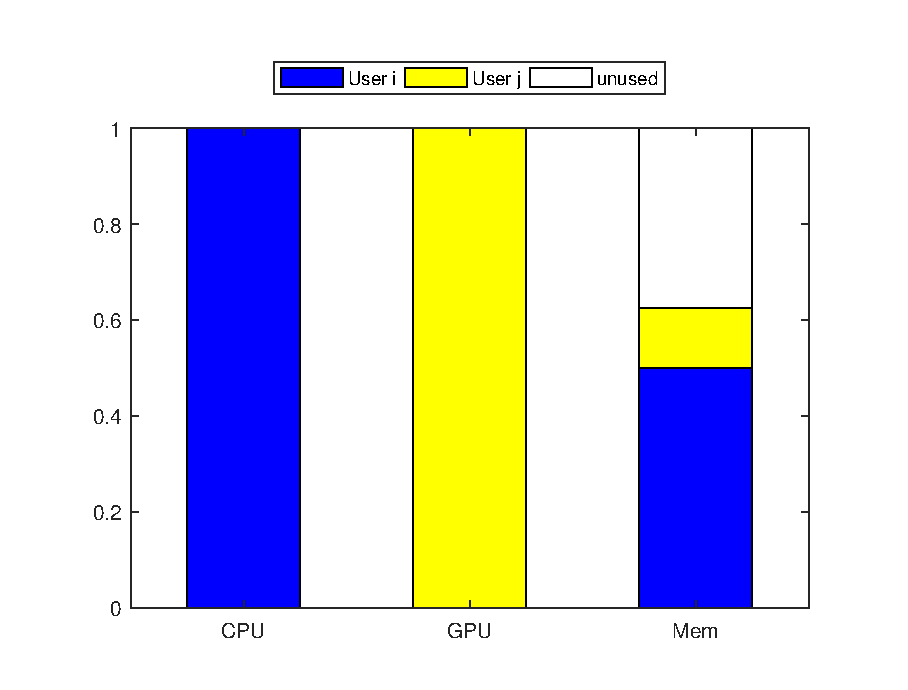
\includegraphics[width=0.8\linewidth]{figs/DRF-threshold}
% 	\caption{All CPU cores belongs to User $i$ based on DRF. The allocation is still worse than equal sharing for User $i$ as 128 CPU cores worth less than 4 GPUs for User $i$. }
% 	\label{fig:DRF-threshold}
% \end{figure}


% \begin{figure}
% 	\centering
% 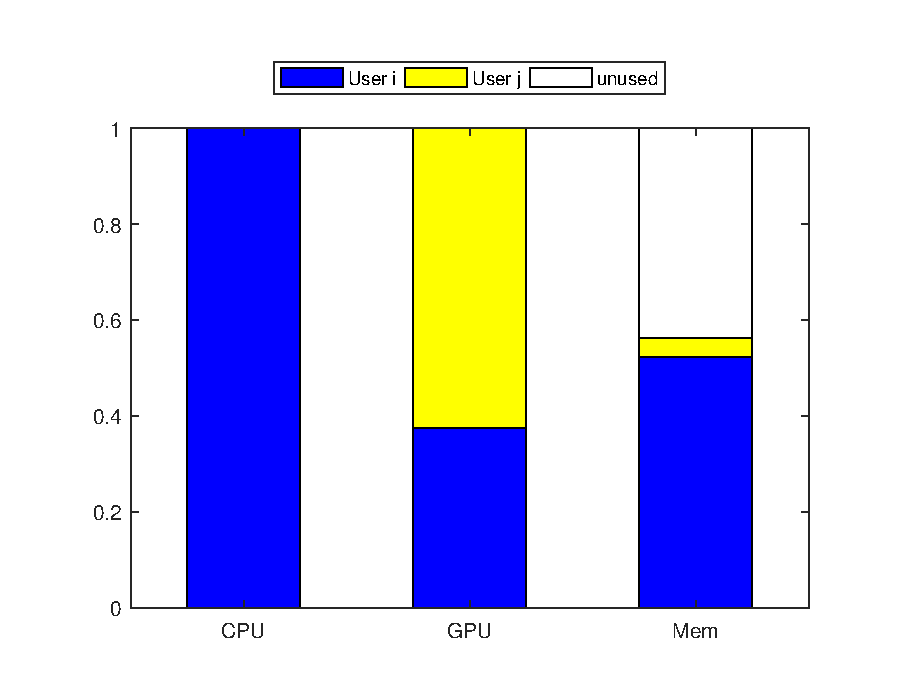
\includegraphics[width=0.8\linewidth]{figs/DRF-merge}
% 	\caption{All CPU cores belongs to User $i$ based on DRF. The allocation is still worse than equal sharing for User $i$ as 128 CPU cores worth less than 4 GPUs for User $i$. }
% 	\label{fig:DRF-merge}
% \end{figure}

\subsubsection{Our idea}
\label{sec:fairness_score}

\name maintains a progress for each user over time. Whenever a resource becomes available, \name schedules jobs from users with lower progress for fairness. The key is therefore how to update the progress measure over time.  
For job $i$, it has the CPU configuration $(c, m_c, p_c)$, where $c$ is the CPU demand, $m_c$ is the memory demand, and $p_c$ is the processing time on CPU, and the GPU configuration $(g, m_g, p_g)$, where $g$ is the GPU demand, $m_g$ is the memory demand, and $p_g$ is the processing time on GPU. 

If $p_c$ is smaller than $p_g$ (CPU is more effective), we use the dominant share of the CPU configuration $d_i=\max\{c/C, m_c/M\}$, where $C$ and $M$ are the CPU and memory capacity of the cluster. 
Otherwise, we use the dominant share of the GPU configuration $d_i=\max\{g/G, m_c/M\}$, where $G$ is the GPU capacity of the cluster. 

The (instantaneous) value of the job $i$ is based on the dominant share, but discounted if the job is not placed on the more effective resource. For instance, if job $i$ is more effective on GPU but is placed on CPU, its value $v_i = \frac{p_g}{p_c} d_i = \frac{p_g}{p_c} \max\{g/G, m_g/M\}$. A user's progress is the sum of values of all her jobs that are currently running.

%We define the progress of a user based on instantaneous dominant share.  
% The idea is the following: Every user wishes his/her jobs to be finished as fast as possible. But sometimes, that is not doable as some jobs have to sacrifice and take the suboptimal configurations for the performance of other jobs. The system shouldn't punish them for taking a suboptimal solution and finish slower.\mosharaf{Unclear what it means.} For example, assume a job can finish within 5 mins on GPU or 20 mins on CPU, the CPU unit time/score of the job should be $\frac{1}{4}$ of the GPU counterpart.

% \xiao{I rewrote above paragraph}

%The idea is the following: 
% As each job has two configurations with different processing times.  From users perspective, they all prefer to pick the configuration that results in a better completion time. However, this is not always possible, as there might be intense competitions among users from their favorite resource in a cluster. As a consequence, some jobs have to sacrifice and take the suboptimal configurations for discounted progress. For example, assume a job can finish within 5 mins on GPU or 20 mins on CPU, the CPU unit time/progress of the job is $\frac{1}{4}$ of the GPU counterpart.




% score $v(i)$ for a single job $i$ will be calculated only when the job is being processed.

% From the configuration matrix $$
% Q_i=
% \begin{bmatrix}
% c_i & m_i^1 & p_i^1 \\
% g_i & m_i^2 & p_i^2 
% \end{bmatrix} $$

% Let the faster configuration in the matrix be $(x_i,m_i,p_i)$. Let the dominant share of this configuration be $d_i$, where
% \[
% d_i=
% \begin{cases}
% \max(\frac{x_i}{C_1},\frac{m_i}{C_3}), & p_i^1 \leq p_i^2 \\
% \max(\frac{x_i}{C_2},\frac{m_i}{C_3}), & p_i^1 > p_i^2
% \end{cases}
% \]


% Then

% \[
% v_i=
% \begin{cases}
% \frac{p_i}{p^1_i}d_i, & \mbox{If job $i$ placed on CPU} \\
% \frac{p_i}{p^2_i}d_i, & \mbox{If job $i$ placed on GPU}
% \end{cases}
% \]


% % simply compare $p_i^1$ and $p_i^2$ and check the placement of job $i$. \begin{itemize}
% % 	\item If $p_i^1 <  p_i^2$, and job $i$ is placed on CPU, then $v(i) = \max(\frac{c_i}{C_1},\frac{m_i^1}{C_3})$;
% % 	\item If $p_i^1 <  p_i^2$, and job $i$ is placed on GPU, then $v(i) = \frac{p_i^1}{p_i^2}\max(\frac{c_i}{C_1},\frac{m_i^1}{C_3})$;
% % 	\item If $p_i^1 \geq  p_i^2$, and job $i$ is placed on CPU, then $v(i) = \frac{p_i^2}{p_i^1} \max(\frac{g_i}{C_2},\frac{m_i^2}{C_3})$;
% % 	\item If $p_i^1 \geq  p_i^2$, and job $i$ is placed on GPU, then $v(i) = \max(\frac{g_i}{C_2},\frac{m_i^2}{C_3})$;
% % \end{itemize} 



% Where $(C_1,C_2,C_3)$ represents the cluster capacity of \\$(CPU,GPU,MEM)$.
% The progress of a user is the sum of all scores from its jobs that are currently being processed. 

%\todo{add explanations}

%The score is a composition of two parts: the preferred configuration, and actual configuration from scheduling. The former decides the dominant share of the job, while the latter decide the scaling of the dominant share

Consider a simple example where the job has CPU configuration $(1, 4, 20)$ and GPU configuration $(1, 2, 5)$. The system capacity is $(8, 2, 64)$ for CPU, GPU, and memory. 
Because GPU provides a shorter processing time, the dominant share of the job is $\frac{1}{2}$. If the job is actually scheduled on GPU, its value is $\frac{1}{2}$. Otherwise it is discounted by $\frac{1}{4}$ ( to $\frac{1}{8}$) because running on CPU is 4 times slower than GPU. 

Generally speaking, the value of a job is decided by its preferred configuration and the actually resource allocated to it. The former decides the dominant share of the job similar to DRF using the preferred configuration, while the latter decides the speed of consuming that dominant share. In our example, as the job will run 4 times longer on CPU, its (instantaneous) value is divided by 4. Over the execution of the job, either on CPU or GPU, its aggregated value is the same. 
Actually, the progress of a user can be viewed as her instantaneous throughput. %For the example above, and assume the system has 2 identical users. When the progress of two users equal, then either they share both CPU and GPU (i.e, each get 4 CPUs and 1 GPU) or one gets all CPUs and 0 GPU while the other get 2 GPUs. In any case, the throughput speeds of for both users are 2 ($1+\frac{1}{4}\times 4 = \frac{1}{4}\times 8 +0 = 0+2)$.




% $$Q_1 =
% \begin{bmatrix}
% 4 & 4 & 20 \\
% 1 & 4 & 5  \\ 
% \end{bmatrix} $$
% with cluster capacity $(20,10,50)$. Clearly, user prefer GPU as the GPU configuration is 4 times faster than CPU. The dominant share of the job is thus $\frac{1}{10}$. If the job is eventually scheduled on GPU, then the score is also $\frac{1}{10}$; if it is on CPU instead, the score is $\frac{1}{40}$.

% To understand above
% As each job has two configurations with different processing times.  From users perspective, they all prefer to pick the configuration that results in a better completion time. However, this is not always possible, as there might be intense competitions among users from their favorite resource in a cluster. As a consequence, some jobs have to sacrifice and take the suboptimal configurations for discounted progress. For example, assume a job can finish within 5 mins on GPU or 20 mins on CPU, the CPU unit time/progress of the job is $\frac{1}{4}$ of the GPU counterpart.




% Actually, we can prove the following: 

% \begin{restatable}[]{lem}{imposs}  If the progress of all users equal, then the allocation is envy-free, moreover, if either computation or memory is used up, the allocation is Pareto-efficient and sharing-incentive.\end{restatable}

% The intuition behind the lemma is that the progress is a way to measure 'effective resource' a user receive, if the score is same for all users, then they are treated equally by the system.

\subsubsection{Incorporating fairness into \name}

%Given the fairness system we designed in section 4.2, we can use the progress to evaluate how much resource is being used by a user at the current time. Then clearly we should prioritize users with lower progress.

\name provides a fairness knob and the system operator can adjust its value $\alpha$ in $[0,1]$, which affects how many users are taken into consideration when a scheduling is triggered. For instance, with 20 users and $\alpha = 0.3$, only jobs from 6 users with lowest progress are considered for scheduling. When $\alpha=1$, there is no fairness constraint and all users are considered. The \name algorithm is based on Algorithm~\ref{alg:greedy} and incorporates online arrivals and fairness considerations. 

%\todo{Add the Allox algorithm formal description with fairness consideration}
%\xiao{I edited the algorithm as the following with some extra explanations}
\begin{algorithm}[H]
\small
\caption{\name Scheduler}
\label{alg:allox_scheduler}
\begin{algorithmic}[1]
	\Function{ScheduleNextJob}{available machine $i$}
    \State {Update users' progress and get the set of users $A_{\alpha}$ consisted of $\ceil*{\alpha n}$ users with the lowest progress.} %whose fairness score is within $\ceil*{\alpha n}$ of all users}
    \ForAll{job $j$ in the waiting queue from $A_{\alpha}$}
    \State Add processing time of job $j$ to matrix $P$
    \EndFor
    \State Generate the delay matrix $D$ and further the cost matrix $Q$;
    %\State Generate cost matrix $Q$ using  equation \ref{eq:generate_cost}
    \State Solve the min-cost matching problem defined by $Q$ to get the matching matrix $M$
    \For{$k = J:1$ } \Comment{$J$ is the total \# of jobs in $A_{\alpha}$}
      \For {$w = 1:J$}
        \If{$M(w,m(k-1)+i) = 1$} \Comment{$w$ is first job scheduled on machine $i$}
          \State schedule job $w$ to machine $i$
          \State Update available time $\omega_i$ and users' progress
          %\State Update users' progress %$v_{j \in u}(u)$
          \State \Return job $w$
      % 	\State Break
        \EndIf
      \EndFor
    \EndFor
	\State \Return null
    \EndFunction
%     \State Generate matrix $Q$;
%     \State Solve a min-cost bipartite matching problem for matrix $Q$;
%     \State Retrieve scheduling from the solution
\end{algorithmic}
\end{algorithm}
%\xiao{ new explanations}

Lines 2-6 of Algorithm~\ref{alg:allox_scheduler} are preparing the input for the matching problem. In particular, it only considers jobs from $\ceil*{\alpha n}$ users with the lowest progress. 
After solving the min-cost matching problem in Line 7, the algorithm simply searches for the first job scheduled on machine $i$. 
%In the above scheduling part (line 8-18), the solver for matching problem is the same as in Algorithm 1, but when the scheduler gets the matching matrix $M$, it only schedules 1 job. 
Specifically, the scheduler checks all entries affiliated with the available machine $i$ and find a valid entry with largest $k$, which implies that the corresponding job $w$ is scheduled first according on machine $i$. Recall that $k$ represents the last $k$-th job on a machine. Therefore, the larger $k$ is, the earlier the job is scheduled on that machine.

Occasionally, the scheduler cannot find a valid job. It occurs when no job is scheduled on the available machine based on current jobs and system load. Consider a simple example with 2 jobs, both have 1 minute processing time on GPUs and 10 minutes processing time on CPUs. Assume the cluster has only 1 CPU and 1 GPU. After the scheduler places any job on the GPU, even though the CPU is available, the optimal schedule for the other job is to wait. In this case, the algorithm returns no job and the system waits until the next event such as new job arrivals or a new machine becomes available. For instance, with no new jobs, after 1 minute, the GPU becomes available, and the remaining job will be scheduled on the GPU.





	\section{{\name} Implementation}
\label{sec:system}

%\subsection{System Design}

% \desc{Why do people need Allox?}

% In existing resource managers such as Kubernetes, a job submitted in one configuration cannot be executed on other sources.
%To the best of our knowledge, \name is the first resource allocation system allowing multiple job configurations.
We build \name based on Kubernetes using roughly 3000 lines of Go code for the resource manager and 1500 lines of Python for its online job estimation tool.
We pick Kubernetes because it well supports clusters consisted of heterogeneous resources such as CPU and GPU.

\name has three main components: \emph{Estimator}, \emph{Scheduler}, and \emph{Placer}.
\name first uses the estimator to obtain job characteristics.% of machine learning jobs.% is implemented as in (\S\ref{sec:res_estimation}). 
%The configurations and speed-up rates are fed as input to Scheduler.
The scheduler then uses the algorithm described in the previous section to decide which job to be scheduled next and whether to place it on CPU or GPU.
%The scheduler then decides which jobs to be executed.
Finally, the placer executes the schedule in the system. %the scheduled jobs on the right resource (CPU or GPU). 
The \name system is depicted in Figure \ref{fig:design}.

%\paragraph{Multi-resource Manager}
\begin{figure}
	\centering
	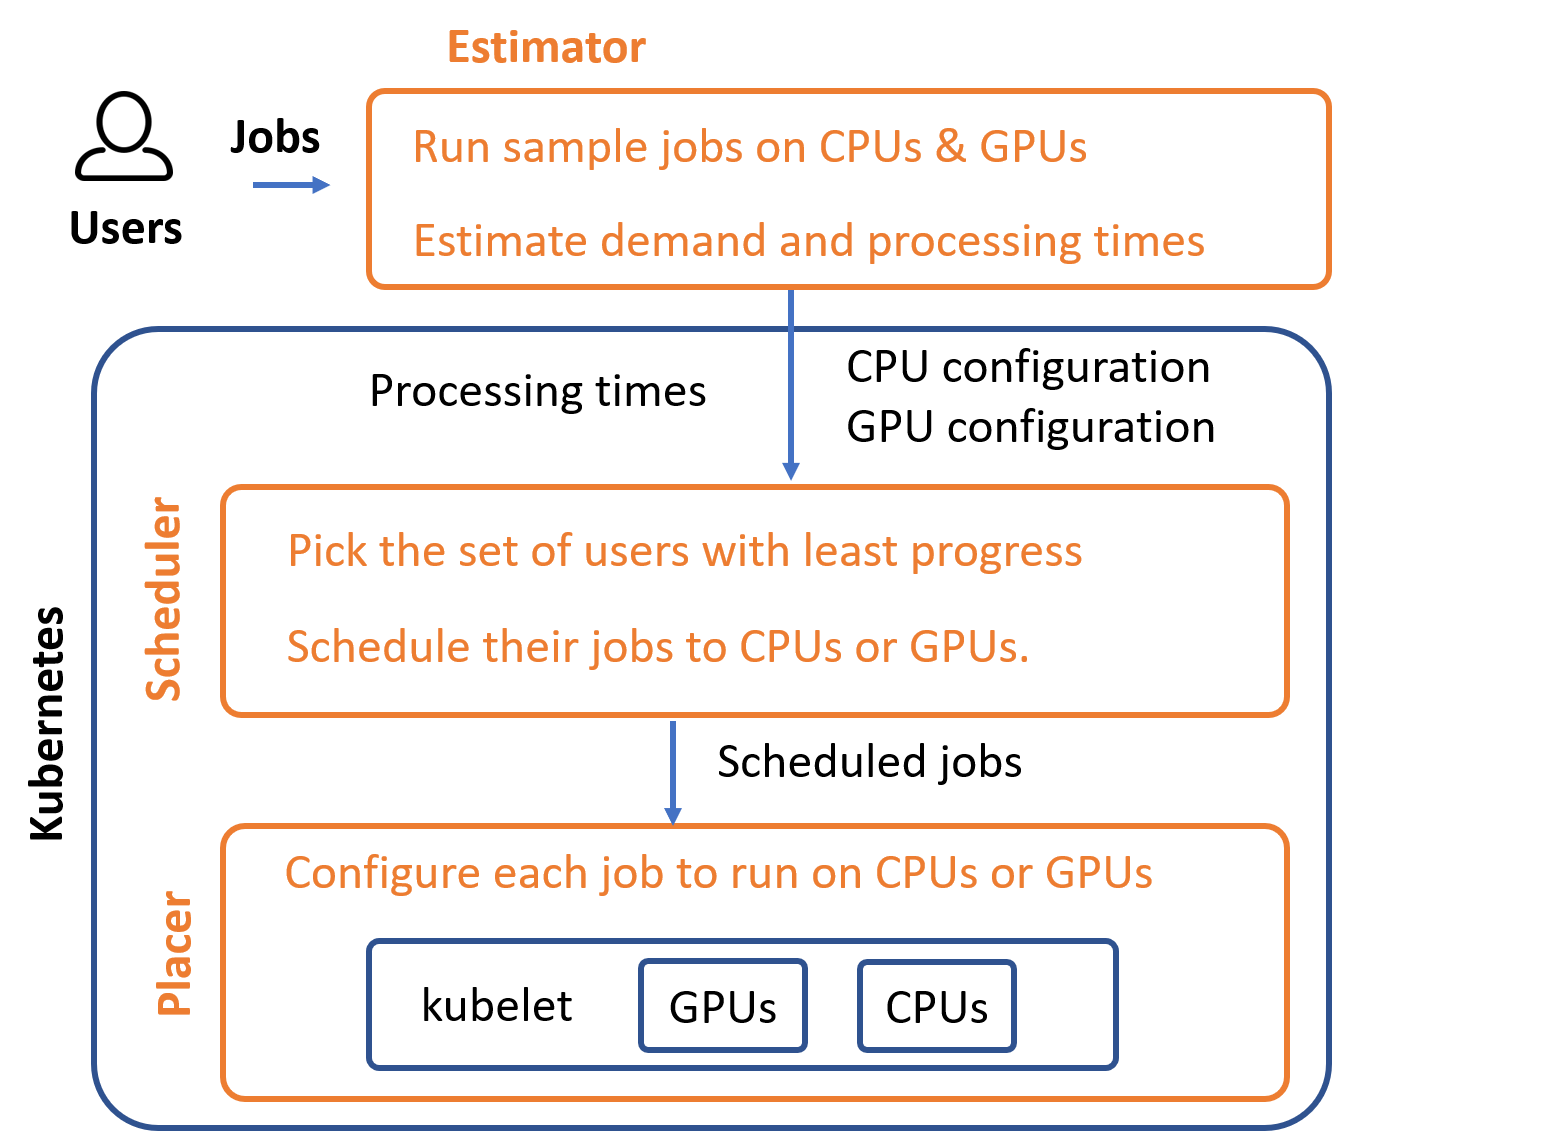
\includegraphics[width=1.0\linewidth]{figs/design}
	\caption{The \name system has three main components: Estimator, Scheduler, and Placer.}
	\label{fig:design}
\end{figure}

\subsection{Estimator}\label{sec:profiling}
%\emph{Estimation Tool}. 
The estimator predicts jobs' resource demands and their processing times on CPU and GPU in an online manner. %to provide information necessary for the schedule to make decisions.
%Users use to submit their jobs via the estimation tool.
For each job, it creates four samples of the job -- two for CPU and the others for GPU -- that are much smaller than the original job.
In our experiment, the total length of the sample jobs is 3\% of the real jobs. While the real jobs can run for hours, the samples last from 30 seconds to 2 minutes. 
Based on the completion time of the samples, we estimate the processing time of the real job on both CPU and GPU. The estimation is relatively accuracy, especially for most machine learning jobs that are iterative~\cite{ernest, slaq_socc17}. 
Figure~\ref{fig:prediction_errors_cdf} shows the CDF of estimation errors of 40 jobs through real experiments. The mean absolute error is 8\% and the standard deviation is 11\%. 

\begin{figure}[h]
	\centering
	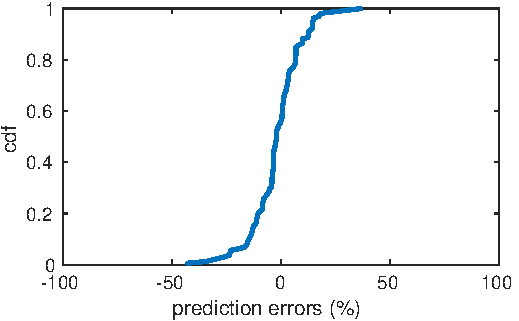
\includegraphics[width=0.7\linewidth]{figs/prediction_errors_cdf}
	\caption{CDF of the estimation errors from experiments.}
	\label{fig:prediction_errors_cdf}
\end{figure}


% Figure \ref{fig:est_compl_time} shows that the completion time of TensorFlow benchmark jobs on GPU are proportional to number of batches.
% \begin{figure}[h]
%   \centering
%   %    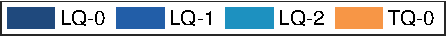
\includegraphics[width=0.6\linewidth]{fig/b1i3_res_usage_legend}
%   {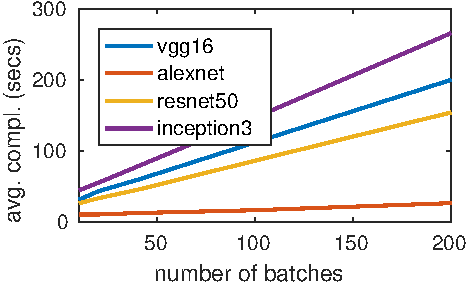
\includegraphics[width=0.7\linewidth]{figs/prof-batchnum-gpu} \label{fig:prof-batchnum-gpu}}    \hspace{0.0in}
%   \caption{(a) The completion times of jobs linearly increase with respect to number of batches.}
%   \label{fig:est_compl_time}
% \end{figure}

%The estimation tool estimates the job completion time using a pair of samples.
%Each sample is a scale version of the job.


% \begin{figure}[!h]
%   \centering
%   \subfloat[] {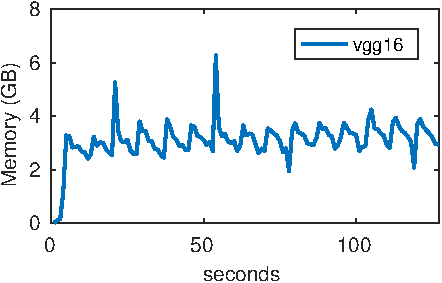
\includegraphics[width=0.45\linewidth]{figs/mem_usage_logcpu} \label{fig:mem_usage_logcpu}}    \hspace{0.1in}
%   \subfloat[] {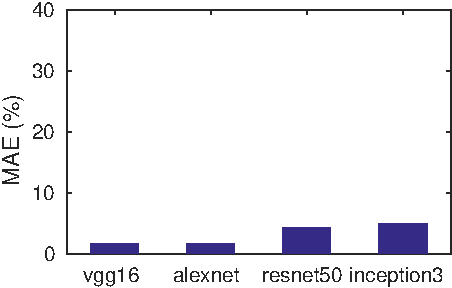
\includegraphics[width=0.45\linewidth]{figs/mem_usage_errcpu} \label{fig:mem_usage_errcpu}}
%   \caption{(a) The memory usage of an ML job has a similar pattern overtime (b) Averaging the memory usage of the short versions can estimate the memory usage average of the job at high accuracy.}
%   \label{fig:mem_usage}
% \end{figure}

% \desc{picking memory}

Similar to Gandiva \cite{gandiva_osdi18}, the estimator determines the memory demands of jobs by monitoring the memory usage of their corresponding samples. 
% As shown in Figure~\ref{fig:mem_usage}, using the sample can predict job's memory demand with acceptable accuracy.

% \desc{picking GPU}

Currently, GPUs do not support fine-grain sharing among multiple jobs \cite{gandiva_osdi18}.
Therefore, a job needs to use a whole GPU in \name. %, a GPU is not shared by multiple jobs in \name, and a job's GPU configuration needs an integral number of GPUs. 
% normally needs a whole GPU.
%A GPU is often powerful enough to carry an ML job.
%If a ML job is paralleled on multiple GPUs, we can consider it as multiple independent jobs.

%Although GPU memory can be statically shared but this results in worse performance due to memory contention.
%Furthermore, GPU memory is limited so ML jobs prefer to fully utilize the GPU memory for their performance.
%ML job and multiple GPUs are not performance effective when they do not support peer-to-peer transfers.
% \desc{picking CPU}
For CPU, the estimator picks the maximum number of cores in a CPU to optimize the performance of the job on CPU.
% Figure \ref{fig:cpu_cores} shows that the performance of TensorFlow jobs is much better using more CPU cores.
As Kubernetes does not allow a container to have more than 1 CPU, \name does not give more CPU cores than a single physical CPU has.
% \begin{figure}[!h]
%   \centering
%   \subfloat[vs. a single CPU core] {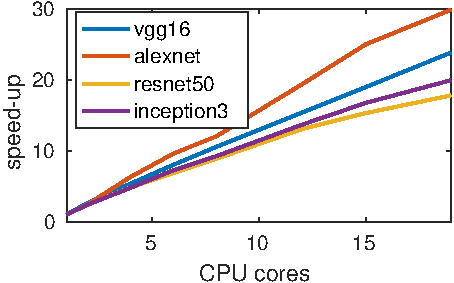
\includegraphics[width=0.7\linewidth]{figs/prof_cpu_speedup} \label{fig:prof_cpu_speedup}}    \hspace{0.1in}
%   %     \subfloat[] {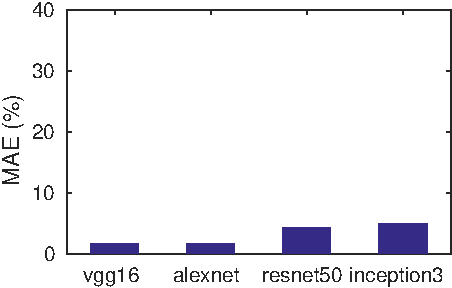
\includegraphics[width=0.45\linewidth]{figs/mem_usage_errcpu} \label{fig:mem_usage_errcpu}}
%   \caption{Users prefer to use more CPU cores as using them significantly improve jobs v.s. using a core.}
%   \label{fig:cpu_cores}
% \end{figure}


\subsection{Scheduler}
%\desc{Scheduler}
%We enable fair resource allocation and job scheduling on Kubernetes scheduler.
Kubernetes does not support fair allocation or job scheduling. As a result, we cannot simply modify some existing scheduler for our algorithm. 
%Given the allocation and CPU/GPU configurations,
%the scheduler chooses which jobs to be scheduled on CPU or GPU.
Instead, we implement our scheduler from scratch using the \textit{kube-scheduler} API.



%The scheduler is mainly implemented by customizing in \textit{kube-scheduler}.
%Although we borrow some fundamental APIs from \textit{kube-scheduler}, several features are significantly changed.

% We add job scheduling in \textit{kube-scheduler}.
% There is a single queue for all available jobs (a.k.a. pods).
% Allocating resources to a pod may take a few seconds in the distributed systems.
% If there are many pods queued up, waiting time in the queue can be large. 
% To allocate resources the pods quickly, \textit{kube-scheduler} schedules pods in an asynchronous manner.
% The scheduler keeps popping pods out of the queue whenever a new pod arrives.
% If a pod is not successfully admitted, it will be added to the queue.
% Basically, the queue has maximum one element at any time.
% However the scheduler requires multiple jobs in the queue so that they pick the best one.
%\todo{Tan, add what you changed \textit{kube-scheduler} to implement the scheduler. DONE} 
Jobs arrive in a single queue in \textit{kube-scheduler}.
Given the set of available jobs, the scheduler decides which job to run. 
\textit{kube-scheduler} receives the estimated processing times of the CPU and GPU configurations from the estimator and passes them to \name scheduler via \textit{kubectl}. 
\name scheduling procedure is activated prior to \textit{Pod Admission}.
%\textit{Pod Admission} then forwards the job to an appropriate node.
If the job is not admitted, it is sent back to the waiting queue.
% The job is picked such that it minimizes the average completion time maintain fairness among users as we present in \S~\ref{sec:alg}.
In addition to our scheduling algorithm, we implement other methods described in Section~\ref{sec:baselines}.

We add fairness support to \textit{kube-scheduler} by updating the progress of all users over time \S~\ref{sec:fairness_score}.
\textit{schedulerCache} in \textit{kube-scheduler} captures the snapshot of the whole system.
When there is an update from the system, \textit{schedulerCache} is notified and \name checks if a job gets resources or finishes.
If a job receives allocated resources, the progress of that user is increased accordingly.
Recall that if a job is running with the unfavorable configuration (with longer processing time), the progress increase is discounted.% from the that of running on the favorable configuration. 
If a job finishes, we deduct its progress from the corresponding user.

%\todo{Tan, add what you changed \textit{kube-scheduler} for fairness.  -- DONE} 

%The key idea of \textit{kube-scheduler} is to fit the pods into available resources in the FIFO manner without considering user resource usage.
%In our scheduler, there are multiple users and a user is mapped to a \textit{namespace} in \textit{kube-scheduler}.
%As a job can be allocated in either on CPU or GPU, fairness cannot rely on resource usage.
%We have our fairness score that actually can generalize the resource usage fairness.


\subsection{Placer}
The placer \emph{dynamically} configures proper containers and executes jobs within these containers.
In the current Kubernetes system, jobs are configured to run on CPU or GPU ahead of time; hence, they do not need the placer.
This is another new component added.% to the current Kubernetes system.

\subsection{Operational issues}

\paragraph{Minimum CPU Per Job}
When developing our scheduler, we realized all jobs running on GPUs also require (a small amount of) CPU for proper execution.
\name addresses this by reserving a small number (one by default) of CPU cores for GPU jobs.%; e.g., we can reserve 1 CPU cores for each GPU.
As the number of CPU cores in a cluster is often large, this change has little impacts on the performance.

\paragraph{Job profiling overhead}
Before a job is scheduled, its sample jobs must be completed first. 
To this end, \name prioritizes all sample jobs. 
Because these sample jobs are relatively small, the overhead is minimal.  
\name also sets a limit on resources for sample jobs to reserve enough resources for the real jobs. In addition, if a sample job is significantly longer than others, we do not need to complete it as it already indicates the original job is very long. We can adjust the sample job size to balance the overheads and estimation accuracy.

\paragraph{Low utilization with small $\alpha$ }
The fairness parameter, $\alpha$, allows the explicit tradeoff between fairness and performance.
However, when $\alpha$ is small, the small set of users may not have jobs or want to wait for better resources, e.g., there are available CPUs but they prefer to wait for GPUs.
%However, these users may not want to execute their jobs on the available machines.
This results in low resource utilization.
To deal with this, \name temporally increases $\alpha$ to include more users who need the available resources.
%If resources (CPUs or GPUs) are still available, we do this until all users are considered, i.e., $\alpha \geq 1$.

\paragraph{Resource availability}
%\name relies on estimated completion times to know when a node will become available, which is needed for the scheduling algorithm.
While it is sufficient to use estimated processing times in the scheduling algorithm, resource availability needs to be obtained separately over time because there may be significant estimation errors. 
%Since there are estimation errors, the availability times are not the same as expected.
%In this case, \name needs to know the availability of machines. 
By default, Kubernetes periodically checks the health and updates from each node. Therefore, resource availability can be collected together with the current health check without additional overheads. %the events if the nodes are healthy and updates the (\textit{schedulercache.NodeInfo}).
If we need to inquire the availability information from all nodes very frequently, it might still lead to significant communication overheads for large-scale clusters. In this case, the information of nodes and jobs (\textit{schedulercache.NodeInfo}) are cached in each node and can be updated via events to the master node. 
%Therefore, Kubernetes can periodically checks the events if the nodes are healthy and updates the (\textit{schedulercache.NodeInfo}).
%Meaning, \name can obtain the node availability via \textit{schedulercache.NodeInfo} without creating additional overheads.

%If a job finishes before its expected completion time, we update the corresponding resources' availability.
%If it finishes after, we do not schedule any new jobs on the resources occupied by that job.

\paragraph{Scalability}
The network flow problem for job scheduling can be solved in polynomial time. Using the Hungarian algorithm, the computation complexity is $\mathcal{O}((mn)^3)$ where $m$ is the number of nodes and $n$ is the number of jobs. In a large-scale system with many jobs to schedule simultaneously, this might become the bottleneck.
%\name can be computationally bottlenecked in solving the matching problem for scheduling.
To reduce the complexity, \name picks a subset of jobs instead of the entire queued up jobs based on the processing time on each resource, and it still provides similar performance but with much fast speed. This is validated in Section~\ref{sec:N_max}.
%We limit $N_{max}$, the maximum size of the subset.
%We pick up to $N_{max}$ jobs such that they are either shortest on CPU or GPU.
%Intuitively, \name prefer to schedule the short jobs first.
%We show that small $N_{max}$ still achieves a very close performance to the optimal one in \S\ref{sec:N_max}.
	\section{Evaluation}

\paragraph{Setup.} We use the real-trace workloads from Google.

\emph{Workload}

\emph{Experimental setup}

\emph{Simulation setup}

\paragraph{Metrics}

\subsection{Experimental Results}

\subsubsection{Performance Guarantee}

\subsubsection{Long-term Fairness}

\subsection{Simulations}
	\section{Related Work}
\label{sec:related}

\paragraph{Bursty Applications in Big Data Clusters}
Big data clusters experience burstiness from a variety of sources, including periodic jobs \cite{jockey, rope, scarlett, omega}, interactive user sessions \cite{splunk-analysis}, as well as streaming applications \cite{spark-streaming, millwheel, trident}. 
Some of them show predictability in terms of inter-arrival times between successive jobs (\eg, Spark Streaming \cite{spark-streaming} runs periodic mini batches in regular intervals), while some others follow different arrival processes (\eg, user interactions with large datasets \cite{splunk-analysis}).
Similarly, resource requirements of the successive jobs can sometimes be predictable, but often it can be difficult to predict due to external load variations (\eg, time-of-day or similar patterns); the latter, without {\name}, can inadvertently hurt batch queues (\S\ref{sec:motivation}). 

\paragraph{Multi-Resource Job Schedulers}
Although early jobs schedulers dealt with a single resource \cite{late, mantri, quincy}, modern cluster resource managers, \eg, Mesos \cite{mesos}, YARN \cite{yarn}, and others \cite{omega, borg, cosmos}, employ multi-resource schedulers \cite{drf, sjf, tetris, carbyne, apollo, mercury, hdrf} to handle multiple resources and optimize diverse objectives. 
These objectives can be fairness (\eg, DRF \cite{drf}), performance (\eg, shortest-job-first (SJF) \cite{sjf}), efficiency (\eg, Tetris \cite{tetris}), or different combinations of the three (\eg, Carbyne \cite{carbyne}).
% 
However, \emph{all} of these focus on instantaneous objectives, with instantaneous fairness being the most common goal. 
To the best of our knowledge, {\name} is the first multi-resource job scheduler with long-term memory.

\paragraph{Handling Burstiness}
Supporting multiple classes of traffic is a classic networking problem that, over the years, have arisen in local area networks \cite{cbq, intserv-hierarchy, hfsc, diffserv-rfc2475}, wide area networks \cite{bwe, b4, swan}, and in datacenter networks \cite{silo, qjump}. 
All of them employ some form of admission control to provide quality-of-service guarantees.
They also consider only a single link (\ie, a single resource). 
In contrast, {\name} considers multi-resource jobs and builds on top this large body of existing literature.

BVT \cite{bvt} was designed to work with both real-time and best-effort tasks. Although it prioritizes the real-time tasks, it cannot guarantee performance and fairness.

\paragraph{Expressing Burstiness Requirements}
{\name} is not the first system that allows users to express their time-varying resource requirements. 
Similar challenges have appeared in traditional networks \cite{hfsc}, network calculus \cite{cruz1, cruz2}, datacenters \cite{silo, pulsar}, and wide-area networks \cite{bwe}.
Akin to them, {\name} requires users to explicitly provide their burst durations and sizes; {\name} tries to enforce those requirements in short and long terms. 
Unlike them, however, {\name} explores how to allow users to express their requirements in a multi-dimensional space, where each dimension corresponds to individual resources. 
One possible way to collapse the multi-dimensional interface to a single dimension is using the notion of \emph{progress} \cite{hug, drf}; however, progress only applies to scenarios when a user's utility can be captured using Leontief preferences. 

	\section{Conclusion}
\label{sec:outro}

%We observe that all existing schedulers force the same performance goal on all jobs, which fails to serve both latency-sensitive {\burstq}s and throughput-sensitive {\batchq}s.
%In fact, existing ``fair'' schedulers \cite{drf, drfq, hdrf,jaffe-maxmin} only make instantaneous decisions causing high latency for {\burstq}s.
%On the other hand, just giving high priority to {\burstq}s does not solve the problem because it may starve the \batchq jobs.
To enable the coexist of latency-sensitive {\burstq}s and the {\batchq}s, we proposed \name (Bounded Priority Fairness).
\name provides bounded performance guarantee to {\burstq}s and maintains the long-term fairness for {\batchq}s.
\name classifies the queues into three classes: Hard Guarantee, Soft Guarantee and Elastic.
\name provides the best performance to {\burstq}s in the Hard Guarantee class and the better performance for {\burstq}s in the Soft Guarantee class. The scheduling is executed in a strategyproof manner, which is critical for public clouds. 
The queues in the Elastic class share the left-over resources to maximize the system utilization. 
In the deployments, we show that \name not only outperforms the DRF up to $5.38\times$ for {\burstq} jobs but also protects {\batchq} jobs up to $3.05\times$ compared to Strict Priority. When {\burstq}'s arrivals have different sizes, adding the $\alpha$-strategy can satisfy the deadlines with similar resource utilization.
%The sensitivity analysis shows that our scheduler is robust to estimation errors and non-preemption.

%\nhattan{We need to summarize the properties of BPF here.}

\phantomsection
\label{EndOfPaper}


%\section{\diff{Potential improvement}}

%\subsection{Improve the utilization of \name}

%We observe that \name may result in \emph{low utilization} if the demand \burstq users are highly unbalanced. For example, because \burstq users require more memory than CPU that makes a large amount of memory unallocated like Figure \ref{fig:admission_speedfair_cluster}.

%The idea to allocate resources like HUG \cite{hug} does instead of DRF \cite{drf} for the leftover resources. However, HUG requires the elastic demands and correlated demand vectors. 
%\begin{itemize}
%	\item We can collect the \emph{correlated demand vectors} from each queue. Hence, we can compute HUG for each elastic queue.
%	\item To have something like elastic demands, we need to implement an \emph{inner-queue scheduler} instead of using FIFO. The idea is schedule the queued up jobs in the elastic queues to \emph{utilize their allocated share}. I think this one is not straight forward because the scheduler needs to choose the \emph{best set of jobs to be allocated}.
%\end{itemize}


%\section{\diff{Next steps}}

%\subsection{support subseconds level for burstiness 2DF}

%\subsection{longer tasks}

%\subsection{memory caching}


		
	
	\label{EndOfPaper}
    \newpage
	
	%\input{scripts/todos}
	
	\bibliographystyle{ACM-Reference-Format}
	\bibliography{bib/refs.bib}
	
	\appendix
\section{Appendices}
\subsection{Proof of Lemma \ref{lem:drf_fail}}
Consider a simple case with $n$ users, and each user has identical jobs. The speedup of using a GPU versus a CPU is $(1+\epsilon)$ for all jobs. %times better than a CPU for all jobs.
Clearly, users would choose the configuration that runs faster, which are the GPU configurations in this case. 
By the allocation with DRF, all GPUs are shared equally among users while all CPUs remain idle. Assuming other resources such as the memory is not the bottleneck, the allocation is not Pareto efficient because CPUs can be utilized to improve the progress of all users. 
This allocation does not provide sharing incentive because every user is worse than equal sharing, where each user has some CPUs in addition to the same amount of GPUs allocated.
Finally, if some user lies that she prefers CPUs, she will get all the CPU nodes and progress faster than others. This violates strategy-proofness.


\subsection{Proof of Lemma \ref{lem:imposs}}
Consider two users $A$ and $B$. Both have identical jobs. The speedup of user $A$'s jobs is $\beta_A=2$, while the speedup of user $B$'s jobs is $\beta_B=4$. Assume computation is the bottleneck for both users. The system has the same amount of CPUs and GPUs, normalized to 1. 

We first consider the sharing incentive (SI) and Pareto efficiency (PE) properties. SI requires user $A$ gets at least $\frac{1}{2}(1+2) = \frac{3}{2}$ computational resources (CPUs and GPUs combined), while user $B$ gets at least $\frac{1}{2}(1+4)=\frac{5}{2}$ computational resources. From PE, we know that user $A$ should use CPUs first while user B should use GPUs first because $\beta_A < \beta_B$. 
Because GPUs are more effective, user $A$ should get all the CPUs and some fraction of GPUs. 

Note PE also requires that there should not be any leftover CPUs or GPUs if computation is the system bottleneck. 
Let $A$'s share on GPU be $x$. Then $B$'s share on GPU is $1-x$. By the sharing incentive property, for user $A$, we have $2 x +1 \geq \frac{3}{2}$, i.e., $ x\geq \frac{1}{4}$; for user $B$, we have $4(1-x)\geq \frac{5}{2}$, where we have $x \leq \frac{3}{8}$. Therefore SI and PE requires $\frac{1}{4} \leq x \leq \frac{3}{8}$.
	
If both users report truthfully, assuming at the final allocation, $\exists \delta>0$ s.t. $x+\delta < \frac{3}{8}$, we show it is not strategyproof for user $A$. Specifically, we show that by lying about her speedup ratio, user $A$ can always get at least $(\frac{3}{8}-\sigma)$ fraction of GPU for any small $\sigma > 0$.

To see this, let user $A$ report $\beta'_A = 4- \epsilon$ for some small $\epsilon>0$ instead of the true value $2$. By the SI property, user $A$ needs to get at least $\frac{1}{2}(1+4-\epsilon)$ computational resources. As she has a lower speedup ratio than user $B$, she will get all CPU, therefore the computational resources from GPUs are $\frac{1}{2}(1+4-\epsilon)-1 = 1.5-0.5\epsilon$. This implies that user $A$ needs to get at least $\frac{1.5-0.5\epsilon}{4-\epsilon}$ fraction of GPU, which approaches arbitrary close to $\frac{3}{8}$ with decreasing $\epsilon$. Therefore, there exists an $\epsilon$ that user $A$ can use to get at least $(\frac{3}{8}-\sigma)$ fraction of GPU. 
Thus, to make sure user $A$ has no incentive to lie, the allocation has to provide at least $\frac{3}{8}$ fraction of GPU to user $A$. 

Similarly, user $B$ can report $\beta'_B=2+\epsilon$ to increase her allocation on GPUs. If she reports $\beta'_B=3$, $B$ can get at least $\frac{2}{3}$ GPU. Clearly, there is not enough GPU to share as $\frac{3}{8} + \frac{2}{3} > 1$. So no allocation can be strategyproof.



% To see this, let $A$ report $\beta'_A = 4- \epsilon$ instead, 
% Consider $A$ report $\beta_A = 4- \epsilon$, for small $\epsilon > 0$, then by SI property, for $A$, she will get all CPU and $f(\epsilon)=\frac{0.5(5-\epsilon)-1}{4-\epsilon} = \frac{1.5-0.5\epsilon}{4-\epsilon}$ fraction of GPU, which is a decreasing function w.r.t. $\epsilon$, and it approaches to $\frac{3}{8}$. By choosing $\epsilon$ s.t. $f(\epsilon)> x+\delta$, we have a larger fraction of GPU compared to truthful reporting. So we have $\forall \delta>0$, $x+\delta \geq \frac{3}{8}$.
	
% 	However, if $A$ gets that much GPU by truthfully reporting $\beta_A = 2$, then $B$ can also game the system by exploiting SI property. $B$ can simply report  $\beta=2+\epsilon$ for a small $\epsilon >0$ from true $\beta_B = 4$ and a bit more memory to achieve better utility. If reported $\beta_B'$ = 3, then $B$ can have at least $\frac{2}{3}$ GPU. Then clearly, there is not enough GPU to share as $\frac{3}{8} + \frac{2}{3} > 1$. So no allocation can be strategyproof.



% \subsection{Proof of Lemma \ref{lem:thresholdDRF}}
% \label{sec:lem:thresholdDRF}

% Assume the normalized CPU and GPU demands for user $i$ per job be $(c_i,g_i)$. Let the allocated CPU and GPU for user $i$ be $(a_{1i},a_{2i}$, let the capacity of the CPU and GPU be $(C_1,C_2)$. We show that the solution from the following optimization will produce a solution with desired properties and a threshold $b$.

%  \begin{gather*}
% \max \quad \prod_i z_i \\
% \begin{aligned}
% \textup{s.t.}\quad x_i+y_i  &\leq z_i  & \forall i\\
%                    x_i c_i  &\leq  a_{1i} & \forall i \\
%          y_i g_i  &\leq  a_{2i} & \forall i\\
%          \sum_i a_{1i} &\leq C_1 &~ \\
%          \sum_i a_{2i} &\leq C_2 &~ \\
% \end{aligned}
% \end{gather*}

% We sort the users based on their efficiency $\beta_i = \frac{c_i}{g_i}$ increaingly and firstly we show that $\exists b$ s.t for any user with $\beta_i < b$,  $a_{2i} = 0$ and for 
% any user with $\beta_i > b$,  $a_{1i} = 0$. 



% We show that any CEEI (Competitive Equilibrium from Equal Income) solution will produce a threshold $b$ and the allocation is PE,SI and EF. CEEI provides every user with same amount of toy money and user can buy and trade their resource. When the market reaches competitive equilibrium, the ratio of unit price per GPU and unit price per CPU is the threshold we need.  The formulation can be written as the following, where $x_i$ and $y_i$ represents the number of jobs to be scheduled as CPU configurations and GPU configurations respectively.
% \begin{gather*}
% \max \quad \prod_i v_i \\
% \begin{aligned}
% \textup{s.t.}\quad x_i+y_i  &\leq v_i  & \forall i\\
%                    x_i c_i  &\leq  a_{1i} & \forall i \\
%          y_i g_i  &\leq  a_{2i} & \forall i\\
%          x_im_i^1 + y_im^2_i &\leq a_{3i} & \forall i \\
%          \sum_i (a_{1i},a_{2i},a_{3i}) &\leq (C_1,C_2,C_3) &~ \\
% \end{aligned}
% \end{gather*}



% The solution can be done via a geometric programming.

% By definition, CEEI is envy-free as each user has the same amount of toy money and the prices for all resources are indiscriminate among users. As the computation is the only bottleneck, the allocation is also Pareto-efficient. The SI comes from free trading among all users.




% Assume that we know  $b$, one may also want to merge CPU and GPU resources into a combined one, i.e., computation resource, and apply the DRF algorithm on this combined resource. Specifically, the system picks $b$ representing the ratio between average efficiency of 1 GPU over 1 CPU core. Consider a cluster with 128 CPU cores, 8 GPUs and 256 GB memory shared by two users, if $b = 64$, the total computation is then $ 128 + 8 \times 64 =  640$ in terms of CPU cores. Based on this approach, each user gets 320 equivalent CPU cores. For instance, user $i$ may get all CPU cores and 3 GPUs while User $j$ gets 5 GPUs.
% Again, the problem is how to choose the threshold $b$. \todo{Xiao, even if you have all $\beta_i$'s perfectly, can you find this threshold?} \xiao{We can, will add later}\mosharaf{Move}

% One way to calculate the $b$ is through CEEI  (Competitive Equilibrium from Equal Income) approach. The system provides every user with same amount of toy money and user can buy and trade their resource. When the market reaches competitive equilibrium, the ratio of unit price per GPU and unit price per CPU is the threshold we need. The solution can be done via a geometric programming. However, this is not practical in the real case. Firstly, the jobs from users may not be homogeneous over time, meaning that with departures and arrivals the efficiency of different users may change sharply, as a consequence, the allocation calculated from CEEI could varies drastically, which is not practical in the real case.\mosharaf{Move}	
	
	
\end{document}\grid
